%% bare_conf.tex
%% V1.3
%% 2007/01/11
%% by Michael Shell
%% See:
%% http://www.michaelshell.org/
%% for current contact information.
%%
%% This is a skeleton file demonstrating the use of IEEEtran.cls
%% (requires IEEEtran.cls version 1.7 or later) with an IEEE conference paper.
%%
%% Support sites:
%% http://www.michaelshell.org/tex/ieeetran/
%% http://www.ctan.org/tex-archive/macros/latex/contrib/IEEEtran/
%% and
%% http://www.ieee.org/

%%*************************************************************************
%% Legal Notice:
%% This code is offered as-is without any warranty either expressed or
%% implied; without even the implied warranty of MERCHANTABILITY or
%% FITNESS FOR A PARTICULAR PURPOSE! 
%% User assumes all risk.
%% In no event shall IEEE or any contributor to this code be liable for
%% any damages or losses, including, but not limited to, incidental,
%% consequential, or any other damages, resulting from the use or misuse
%% of any information contained here.
%%
%% All comments are the opinions of their respective authors and are not
%% necessarily endorsed by the IEEE.
%%
%% This work is distributed under the LaTeX Project Public License (LPPL)
%% ( http://www.latex-project.org/ ) version 1.3, and may be freely used,
%% distributed and modified. A copy of the LPPL, version 1.3, is included
%% in the base LaTeX documentation of all distributions of LaTeX released
%% 2003/12/01 or later.
%% Retain all contribution notices and credits.
%% ** Modified files should be clearly indicated as such, including  **
%% ** renaming them and changing author support contact information. **
%%
%% File list of work: IEEEtran.cls, IEEEtran_HOWTO.pdf, bare_adv.tex,
%%                    bare_conf.tex, bare_jrnl.tex, bare_jrnl_compsoc.tex
%%*************************************************************************

% *** Authors should verify (and, if needed, correct) their LaTeX system  ***
% *** with the testflow diagnostic prior to trusting their LaTeX platform ***
% *** with production work. IEEE's font choices can trigger bugs that do  ***
% *** not appear when using other class files.                            ***
% The testflow support page is at:
% http://www.michaelshell.org/tex/testflow/



% Note that the a4paper option is mainly intended so that authors in
% countries using A4 can easily print to A4 and see how their papers will
% look in print - the typesetting of the document will not typically be
% affected with changes in paper size (but the bottom and side margins will).
% Use the testflow package mentioned above to verify correct handling of
% both paper sizes by the user's LaTeX system.
%
% Also note that the "draftcls" or "draftclsnofoot", not "draft", option
% should be used if it is desired that the figures are to be displayed in
% draft mode.
%
\documentclass[10pt, conference, compsocconf]{IEEEtran}
% Add the compsocconf option for Computer Society conferences.
%
% If IEEEtran.cls has not been installed into the LaTeX system files,
% manually specify the path to it like:
% \documentclass[conference]{../sty/IEEEtran}





% Some very useful LaTeX packages include:
% (uncomment the ones you want to load)


% *** MISC UTILITY PACKAGES ***
%
%\usepackage{ifpdf}
% Heiko Oberdiek's ifpdf.sty is very useful if you need conditional
% compilation based on whether the output is pdf or dvi.
% usage:
% \ifpdf
%   % pdf code
% \else
%   % dvi code
% \fi
% The latest version of ifpdf.sty can be obtained from:
% http://www.ctan.org/tex-archive/macros/latex/contrib/oberdiek/
% Also, note that IEEEtran.cls V1.7 and later provides a builtin
% \ifCLASSINFOpdf conditional that works the same way.
% When switching from latex to pdflatex and vice-versa, the compiler may
% have to be run twice to clear warning/error messages.






% *** CITATION PACKAGES ***
%
%\usepackage{cite}
% cite.sty was written by Donald Arseneau
% V1.6 and later of IEEEtran pre-defines the format of the cite.sty package
% \cite{} output to follow that of IEEE. Loading the cite package will
% result in citation numbers being automatically sorted and properly
% "compressed/ranged". e.g., [1], [9], [2], [7], [5], [6] without using
% cite.sty will become [1], [2], [5]--[7], [9] using cite.sty. cite.sty's
% \cite will automatically add leading space, if needed. Use cite.sty's
% noadjust option (cite.sty V3.8 and later) if you want to turn this off.
% cite.sty is already installed on most LaTeX systems. Be sure and use
% version 4.0 (2003-05-27) and later if using hyperref.sty. cite.sty does
% not currently provide for hyperlinked citations.
% The latest version can be obtained at:
% http://www.ctan.org/tex-archive/macros/latex/contrib/cite/
% The documentation is contained in the cite.sty file itself.




\usepackage{balance}

% *** GRAPHICS RELATED PACKAGES ***
%
\ifCLASSINFOpdf
  % \usepackage[pdftex]{graphicx}
  % declare the path(s) where your graphic files are
  % \graphicspath{{../pdf/}{../jpeg/}}
  % and their extensions so you won't have to specify these with
  % every instance of \includegraphics
  % \DeclareGraphicsExtensions{.pdf,.jpeg,.png}
\else
  % or other class option (dvipsone, dvipdf, if not using dvips). graphicx
  % will default to the driver specified in the system graphics.cfg if no
  % driver is specified.
  % \usepackage[dvips]{graphicx}
  % declare the path(s) where your graphic files are
  % \graphicspath{{../eps/}}
  % and their extensions so you won't have to specify these with
  % every instance of \includegraphics
  % \DeclareGraphicsExtensions{.eps}
\fi
% graphicx was written by David Carlisle and Sebastian Rahtz. It is
% required if you want graphics, photos, etc. graphicx.sty is already
% installed on most LaTeX systems. The latest version and documentation can
% be obtained at: 
% http://www.ctan.org/tex-archive/macros/latex/required/graphics/
% Another good source of documentation is "Using Imported Graphics in
% LaTeX2e" by Keith Reckdahl which can be found as epslatex.ps or
% epslatex.pdf at: http://www.ctan.org/tex-archive/info/
%
% latex, and pdflatex in dvi mode, support graphics in encapsulated
% postscript (.eps) format. pdflatex in pdf mode supports graphics
% in .pdf, .jpeg, .png and .mps (metapost) formats. Users should ensure
% that all non-photo figures use a vector format (.eps, .pdf, .mps) and
% not a bitmapped formats (.jpeg, .png). IEEE frowns on bitmapped formats
% which can result in "jaggedy"/blurry rendering of lines and letters as
% well as large increases in file sizes.
%
% You can find documentation about the pdfTeX application at:
% http://www.tug.org/applications/pdftex





% *** MATH PACKAGES ***
%
%\usepackage[cmex10]{amsmath}
% A popular package from the American Mathematical Society that provides
% many useful and powerful commands for dealing with mathematics. If using
% it, be sure to load this package with the cmex10 option to ensure that
% only type 1 fonts will utilized at all point sizes. Without this option,
% it is possible that some math symbols, particularly those within
% footnotes, will be rendered in bitmap form which will result in a
% document that can not be IEEE Xplore compliant!
%
% Also, note that the amsmath package sets \interdisplaylinepenalty to 10000
% thus preventing page breaks from occurring within multiline equations. Use:
%\interdisplaylinepenalty=2500
% after loading amsmath to restore such page breaks as IEEEtran.cls normally
% does. amsmath.sty is already installed on most LaTeX systems. The latest
% version and documentation can be obtained at:
% http://www.ctan.org/tex-archive/macros/latex/required/amslatex/math/





% *** SPECIALIZED LIST PACKAGES ***
%
%\usepackage{algorithmic}
% algorithmic.sty was written by Peter Williams and Rogerio Brito.
% This package provides an algorithmic environment fo describing algorithms.
% You can use the algorithmic environment in-text or within a figure
% environment to provide for a floating algorithm. Do NOT use the algorithm
% floating environment provided by algorithm.sty (by the same authors) or
% algorithm2e.sty (by Christophe Fiorio) as IEEE does not use dedicated
% algorithm float types and packages that provide these will not provide
% correct IEEE style captions. The latest version and documentation of
% algorithmic.sty can be obtained at:
% http://www.ctan.org/tex-archive/macros/latex/contrib/algorithms/
% There is also a support site at:
% http://algorithms.berlios.de/index.html
% Also of interest may be the (relatively newer and more customizable)
% algorithmicx.sty package by Szasz Janos:
% http://www.ctan.org/tex-archive/macros/latex/contrib/algorithmicx/




% *** ALIGNMENT PACKAGES ***
%
%\usepackage{array}
% Frank Mittelbach's and David Carlisle's array.sty patches and improves
% the standard LaTeX2e array and tabular environments to provide better
% appearance and additional user controls. As the default LaTeX2e table
% generation code is lacking to the point of almost being broken with
% respect to the quality of the end results, all users are strongly
% advised to use an enhanced (at the very least that provided by array.sty)
% set of table tools. array.sty is already installed on most systems. The
% latest version and documentation can be obtained at:
% http://www.ctan.org/tex-archive/macros/latex/required/tools/


%\usepackage{mdwmath}
%\usepackage{mdwtab}
% Also highly recommended is Mark Wooding's extremely powerful MDW tools,
% especially mdwmath.sty and mdwtab.sty which are used to format equations
% and tables, respectively. The MDWtools set is already installed on most
% LaTeX systems. The lastest version and documentation is available at:
% http://www.ctan.org/tex-archive/macros/latex/contrib/mdwtools/


% IEEEtran contains the IEEEeqnarray family of commands that can be used to
% generate multiline equations as well as matrices, tables, etc., of high
% quality.


%\usepackage{eqparbox}
% Also of notable interest is Scott Pakin's eqparbox package for creating
% (automatically sized) equal width boxes - aka "natural width parboxes".
% Available at:
% http://www.ctan.org/tex-archive/macros/latex/contrib/eqparbox/





% *** SUBFIGURE PACKAGES ***
%\usepackage[tight,footnotesize]{subfigure}
% subfigure.sty was written by Steven Douglas Cochran. This package makes it
% easy to put subfigures in your figures. e.g., "Figure 1a and 1b". For IEEE
% work, it is a good idea to load it with the tight package option to reduce
% the amount of white space around the subfigures. subfigure.sty is already
% installed on most LaTeX systems. The latest version and documentation can
% be obtained at:
% http://www.ctan.org/tex-archive/obsolete/macros/latex/contrib/subfigure/
% subfigure.sty has been superceeded by subfig.sty.



%\usepackage[caption=false]{caption}
%\usepackage[font=footnotesize]{subfig}
% subfig.sty, also written by Steven Douglas Cochran, is the modern
% replacement for subfigure.sty. However, subfig.sty requires and
% automatically loads Axel Sommerfeldt's caption.sty which will override
% IEEEtran.cls handling of captions and this will result in nonIEEE style
% figure/table captions. To prevent this problem, be sure and preload
% caption.sty with its "caption=false" package option. This is will preserve
% IEEEtran.cls handing of captions. Version 1.3 (2005/06/28) and later 
% (recommended due to many improvements over 1.2) of subfig.sty supports
% the caption=false option directly:
%\usepackage[caption=false,font=footnotesize]{subfig}
%
% The latest version and documentation can be obtained at:
% http://www.ctan.org/tex-archive/macros/latex/contrib/subfig/
% The latest version and documentation of caption.sty can be obtained at:
% http://www.ctan.org/tex-archive/macros/latex/contrib/caption/




% *** FLOAT PACKAGES ***
%
%\usepackage{fixltx2e}
% fixltx2e, the successor to the earlier fix2col.sty, was written by
% Frank Mittelbach and David Carlisle. This package corrects a few problems
% in the LaTeX2e kernel, the most notable of which is that in current
% LaTeX2e releases, the ordering of single and double column floats is not
% guaranteed to be preserved. Thus, an unpatched LaTeX2e can allow a
% single column figure to be placed prior to an earlier double column
% figure. The latest version and documentation can be found at:
% http://www.ctan.org/tex-archive/macros/latex/base/



%\usepackage{stfloats}
% stfloats.sty was written by Sigitas Tolusis. This package gives LaTeX2e
% the ability to do double column floats at the bottom of the page as well
% as the top. (e.g., "\begin{figure*}[!b]" is not normally possible in
% LaTeX2e). It also provides a command:
%\fnbelowfloat
% to enable the placement of footnotes below bottom floats (the standard
% LaTeX2e kernel puts them above bottom floats). This is an invasive package
% which rewrites many portions of the LaTeX2e float routines. It may not work
% with other packages that modify the LaTeX2e float routines. The latest
% version and documentation can be obtained at:
% http://www.ctan.org/tex-archive/macros/latex/contrib/sttools/
% Documentation is contained in the stfloats.sty comments as well as in the
% presfull.pdf file. Do not use the stfloats baselinefloat ability as IEEE
% does not allow \baselineskip to stretch. Authors submitting work to the
% IEEE should note that IEEE rarely uses double column equations and
% that authors should try to avoid such use. Do not be tempted to use the
% cuted.sty or midfloat.sty packages (also by Sigitas Tolusis) as IEEE does
% not format its papers in such ways.





% *** PDF, URL AND HYPERLINK PACKAGES ***
%
%\usepackage{url}
% url.sty was written by Donald Arseneau. It provides better support for
% handling and breaking URLs. url.sty is already installed on most LaTeX
% systems. The latest version can be obtained at:
% http://www.ctan.org/tex-archive/macros/latex/contrib/misc/
% Read the url.sty source comments for usage information. Basically,
% \url{my_url_here}.





% *** Do not adjust lengths that control margins, column widths, etc. ***
% *** Do not use packages that alter fonts (such as pslatex).         ***
% There should be no need to do such things with IEEEtran.cls V1.6 and later.
% (Unless specifically asked to do so by the journal or conference you plan
% to submit to, of course. )

\usepackage{array}
% \newcolumntype{L}{>{\centering\arraybackslash}m{0.4cm}}
\newcolumntype{C}{>{\centering\let\newline\\\arraybackslash\vspace{3pt}}b{0.7cm}}
\usepackage{caption}
\usepackage{multirow}
\usepackage[table,xcdraw]{xcolor}
\usepackage[printonlyused,withpage]{acronym}
\usepackage{graphicx}
\usepackage{todonotes}


% correct bad hyphenation here
\hyphenation{op-tical net-works semi-conduc-tor}


\begin{document}

\acrodef{HPC}{High Performance Computing}
\acrodef{DAG}{Directed Acyclic Graph}
\acrodef{MPI}{Message Passing Interface}
\acrodef{GML}{Global Machine Learning}
\acrodef{MDS}{Multidimensional Scaling}
\acrodef{DA-MDS}{Deterministic Annealing Multidimensional Scaling}
\acrodef{SVM}{Support Vector Machine}
\acrodef{LDA}{Latent Dirichlet Allocation}
\acrodef{JVM}{Java Virtual Machine}
\acrodef{ABDS}{Apache Big Data Stack}
\acrodef{JDK}{Java Development Kit}
\acrodef{FJ}{Fork-Join}
\acrodef{LRT-FJ}{Long Running Threads Fork-Join}
\acrodef{LRT-BSP}{Long Running Threads Bulk Synchronous Parallel}
\acrodef{BSP}{Bulk Synchronous Parallel}
\acrodef{CAS}{compare-and-swap}
\acrodef{CPU}{central processing unit}
\acrodef{dTLB}{data Translation Lookaside Buffer}
\acrodef{OS}{Operating System}
\acrodef{NUMA}{Non-Uniform Memory Access}
\acrodef{ccNUMA}{Cache Coherent Non-Uniform Memory Access}
\acrodef{GCC}{GNU Compiler Collection}
\acrodef{DL}{Deep Learning}
\acrodef{SMACOF}{Scaling by MAjorization of a COmplicated Function}
\acrodef{TCP}{Transmission Control Protocol}
\acrodef{GC}{Garbage Collection}
\acrodef{API}{Application program interface}
\acrodef{JIT}{Just In Time}
\acused{HTML}
%
% paper title
% can use linebreaks \\ within to get better formatting as desired

%\title{Optimizing Java Performance on Multicore HPC Clusters for Big Data Anlytics}
\title{Java Thread and Process Performance for Parallel Machine Learning on Multicore HPC Clusters}


% author names and affiliations
% use a multiple column layout for up to two different
% affiliations

\author{\IEEEauthorblockN{Saliya Ekanayake, Supun Kamburugamuve, Pulasthi Wickramasinghe, Geoffrey C. Fox}
\IEEEauthorblockA{School of Informatics and Computing\\
Indiana University, Bloomington\\
sekanaya@indiana.edu, skamburu@indiana.edu, pswickra@indiana.edu, gcf@indiana.edu}}

% conference papers do not typically use \thanks and this command
% is locked out in conference mode. If really needed, such as for
% the acknowledgment of grants, issue a \IEEEoverridecommandlockouts
% after \documentclass

% for over three affiliations, or if they all won't fit within the width
% of the page, use this alternative format:
% 
%\author{\IEEEauthorblockN{Michael Shell\IEEEauthorrefmark{1},
%Homer Simpson\IEEEauthorrefmark{2},
%James Kirk\IEEEauthorrefmark{3}, 
%Montgomery Scott\IEEEauthorrefmark{3} and
%Eldon Tyrell\IEEEauthorrefmark{4}}
%\IEEEauthorblockA{\IEEEauthorrefmark{1}School of Electrical and Computer Engineering\\
%Georgia Institute of Technology,
%Atlanta, Georgia 30332--0250\\ Email: see http://www.michaelshell.org/contact.html}
%\IEEEauthorblockA{\IEEEauthorrefmark{2}Twentieth Century Fox, Springfield, USA\\
%Email: homer@thesimpsons.com}
%\IEEEauthorblockA{\IEEEauthorrefmark{3}Starfleet Academy, San Francisco, California 96678-2391\\
%Telephone: (800) 555--1212, Fax: (888) 555--1212}
%\IEEEauthorblockA{\IEEEauthorrefmark{4}Tyrell Inc., 123 Replicant Street, Los Angeles, California 90210--4321}}




% use for special paper notices
%\IEEEspecialpapernotice{(Invited Paper)}




% make the title area
\maketitle


\begin{abstract}
\texcocolor{blue}{TODO: revise this to say we looked at MPI, Spark and Flink}
Parallel machine learning is computationally intensive and demands strict latency guarantees. To this end, deploying big data frameworks such as Spark and Flink on \ac{HPC} clusters is of growing interest. These frameworks employ Java processes and threads to exploit distributed and shared memory parallelisms. Typically, they spawn one process per node and create threads leisurely as necessary. However, with a large number of cores and multiple \ac{NUMA} domains per node, it is critical to evaluate performance implications of this hybrid approach as machine learning algorithms are highly sensitive to performance variations of parallel tasks. This paper identifies three principal factors responsible for such behavior and presents strategies to minimize their effects. Performance factors of interest are thread models, affinity patterns, and communication techniques. The paper evaluates these factors against two machine learning algorithms, k-means clustering and \ac{MDS}. Performance results on the latest Intel Haswell \ac{HPC} cluster with 24 and 36 cores per node show significant performance improvement with the right optimizations over these factors. Moreover, this research showcases a performance analysis of machine learning with Spark and Flink based on the findings from k-means and \ac{MDS}.
\end{abstract}

\begin{IEEEkeywords}
machine learning; Java; multicore; NUMA; HPC;
\end{IEEEkeywords}


% For peer review papers, you can put extra information on the cover
% page as needed:
% \ifCLASSOPTIONpeerreview
% \begin{center} \bfseries EDICS Category: 3-BBND \end{center}
% \fi
%
% For peerreview papers, this IEEEtran command inserts a page break and
% creates the second title. It will be ignored for other modes.
\IEEEpeerreviewmaketitle



\section{Introduction} \label{sec:intro}
% no \IEEEPARstart
\textcolor{red}{Remove the angle of "optimizing". This is a performance study and experience -- we look at factors affecting performance of machine learning applications on HPC and apply that experience to understand performance and possible improvements to Flink and Spark}

Parallel machine learning 
 including Hadoop, Spark~\cite{Zaharia:2010:SCC:1863103.1863113}, Storm~\cite{toshniwal2014storm}, and Flink~\cite{carbone2015lightweight}, are written in Java.


In recent years, Java has drawn a great deal of attention due to its application in popular frameworks such as Hadoop, Spark~\cite{Zaharia:2010:SCC:1863103.1863113}, Storm~\cite{toshniwal2014storm}, and Flink~\cite{carbone2015lightweight}. With its growing use in the big data domain, this is a crucial time to evaluate Java performance and optimization strategies, especially within \ac{HPC} environments. Typically data querying style big data jobs are run on cloud environments. However there are other complex data analytics applications with significant computations and strict latency guarantees. \ac{GML} applications~\todo{cite gcf paper on GML} such as \ac{MDS}, \ac{SVM}, PageRank, and Deep Learning are all such examples. Previous studies~\todo{cite Big data in HPC references like [1,2,3]} show \ac{HPC} style architectures and interconnects are better suited for these applications than commodity clouds. Optimizing performance on these modern \ac{HPC} systems, however, brings up numerous technical challenges. Java in particular, where memory and thread management are within the \ac{JVM}'s control, requires explicit tuning to yield high performance. 

This paper presents 3 key optimizations to Java concurrency, affinity, and communication, and applies these techniques to implement two machine learning algorithms, k-means clustering and \ac{MDS}, as well as a parallel matrix multiplication kernel. Evaluating these in a modern Intel Haswell \ac{HPC} cluster equipped with Infiniband interconnect shows significant improvement in performance and scalability. Moreover, we benchmark Flink and Spark and discuss their limitations and possible improvements based on these optimizations. 

The technical contributions of this paper are:
\textcolor{blue}{TODO - list technical contributions}
\begin{itemize}
\item Identification, evaluation, and optimization of factors affecting Java big data analytics. 
\end{itemize}

The rest of the chapters are organized as follows. Section~\ref{sec:apps} introduces \ac{GML} and the three applications used in this research for performance evaluation. Section~\ref{sec:models} presents a comparison of parallel programming models available in big data frameworks. In particular, it compares the classic  message passing model with dataflow programming model and discusses their performance implications on \ac{GML} applications. Section~\ref{sec:factors} elaborates on the three optimizations for concurrency, communication, and affinity. It also identifies a few other factors to consider when developing high-performance Java applications. Section~\ref{sec:evaluation} presents the technical evaluation of these optimizations using k-means clustering, \ac{MDS}, and matrix multiplication. Section~\ref{sec:related} and~\ref{sec:conclusion} present work from others on Java optimizations, and the conclusion.

\section{Comparison of Execution Models} \label{sec:exec_models}
MPI and Big data platform implementations follow two different execution models. The key differences are with the task distribution and communication. MPI is a broader execution model that can support different styles of programming including BSP and many task models. Big data platforms primarily follow the data oriented execution model termed data flow model. Flink explicitly uses a pure data flow execution model while Spark uses distributed data sets (RDD) and operations on top of it which closely resembles the data flow model.  

In dataflow model \todo{cite df} the parallel program is expressed as a \ac{DAG}. Parallel tasks are assigned to nodes of the \ac{DAG} and the flow of data between nodes completes the "wiring". In contrast, classic parallel applications employ the message passing model, where long running tasks are orchestrated using point-to-point and collective communication calls.

With MPI machine learning applications, the complete program is executed in a set of pre-allocated tasks that defines the parallelism of the execution. The same tasks do the entire computing and communications required for the program. In contrast to the MPI approach, data flow applications allocate different tasks for different stages of the application connected by communication links. These tasks and communication links forms the execution graph. MPI  programming model permits complete control over the execution in a single task including memory management and thread execution. The data flow execution model hides these details from the user and provides a high level API. 

With current implementations of big data frameworks, programming models and execution models are coupled together even though they can be independent of each other. For example the data flow programming models in Spark and Flink are implemented as data flow execution graphs compared to an in-place execution as in MPI applications.

It is important to note the differences in how the iterations are handled. With data flow applications, iterations are handled as unrolled for loops. Even though the user specifies a for loop execution, it translates to a long graph of data flow. This means the data from one loop's tasks to the next needs to be sent through communications. The MPI model doesn't have this requirement because a for loop is a regular in memory loop in a normal program and the data from the iteration is available to the next via task memory. 

\begin{figure}[!h]
\centering
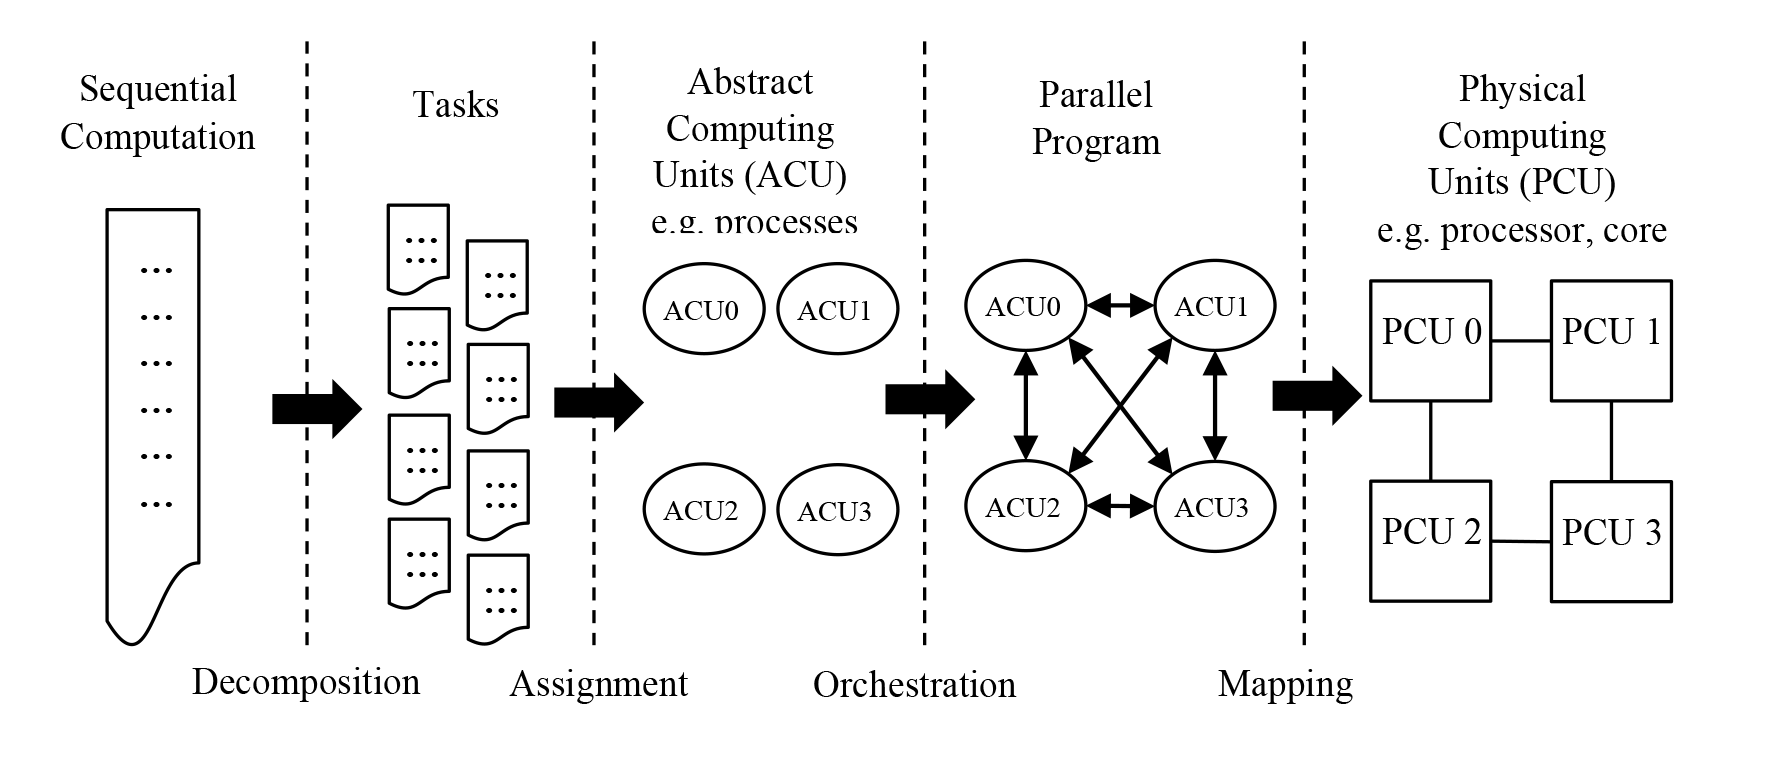
\includegraphics[width=0.9\columnwidth]{images/fig_parallel_decompose}
\caption{Steps of creating a parallel program
\label{fig:fig_steps_of_creating_a_parallel_program}}
\end{figure}

\textcolor{blue}{TODO - a comparison of the classic message passing model to dataflow (or model parameter flow)}

\section{Performance Factors} \label{sec:factors}

Performance of parallel machine learning algorithms is sensitive to runtime variations of individual parallel tasks. The following identifies three important aspects of parallel programming and factors responsible for such noise in performance, especially for applications developed in Java.

\subsection{Thread Parallelism}
Threads offer a convenient construct to implement shared memory parallelism. A common pattern used in both big data and \ac{HPC} is the \ac{FJ} thread model. In this approach, a master thread spawns parallel regions dynamically as required. \ac{FJ} regions are implicitly synchronized at the end, after which the worker threads are terminated and only the master thread will continue until a new parallel region is created. Thread creation and termination are expensive; therefore, \ac{FJ} implementations employ thread pools to hand over forked tasks. Pooled threads are long-lived yet short-activated; they release \acs{CPU} resources and switch to idle state after executing their tasks. This model is subsequently referred to as \ac{LRT-FJ} in this paper.Java has built-in support for \ac{LRT-FJ} through its \texttt{java.util.concurrent.ForkJoinPool}~\footnote{https://docs.oracle.com/javase/tutorial/essential/concurrency/forkjoin.html}. Habanero Java~\cite{Imam:2014:HLJ:2647508.2647514}, an OpenMP~\cite{Dagum:1998:OIA:615255.615542}-like implementation in Java, also supports \ac{LRT-FJ} via its \texttt{forall} and \texttt{forallChunked} constructs.

We experimented with another approach to shared memory parallelism, hereafter referred to as \ac{LRT-BSP}. It resembles the classic \ac{BSP} style, but with threads. \figurename~\ref{fig:fig_fj_vs_lrt} depicts a side-by-side view of \ac{LRT-FJ} and \ac{LRT-BSP} models. The notable difference is that in \ac{LRT-BSP}, threads are busy from start to finish of the program, not just within the parallel region as in \ac{LRT-FJ}. The next important difference is the use of explicit synchronization constructs (blue horizontal lines) after non-trivial parallel work (red bars in figure) in \ac{LRT-BSP}. There are constructs such as \texttt{CyclicBarrier} in Java to aid the implementation of these synchronization steps. However, we employed native \ac{CAS} operations and busy loops for performance as well as to keep threads "hot" on cores.  A third difference in \ac{LRT-BSP} is that the serial part of the code (green bars) is replicated across workers, where as in \ac{LRT-FJ} it is executed by just the master thread. Performance results show that despite the replication of serial work in \ac{LRT-BSP}, it does not add any considerable overhead. The reason for this behavior is that in a well-designed parallel application, the serial portions are trivial compared to the parallel work loads and the total amount of memory accesses in \ac{LRT-BSP} is equal to that of \ac{LRT-FJ} for these parts. 

Beyond the differences in the execution model, we observed a significant performance improvement with \ac{LRT-BSP} compared to \ac{LRT-BSP} for parallel Java applications. Analyzing \texttt{perf} statistics revealed that \ac{LRT-FJ} experiences a higher number of context switches, \acs{CPU} migrations, and \ac{dTLB} load/store misses than \ac{LRT-BSP}. In an \ac{MDS} run the factors were over 15x and 70x for context switches and \acs{CPU} migrations. These inefficiencies coupled with the overhead of scheduling threads lead to noise in computation times within parallel \ac{FJ} regions. Consequently, synchronization points become immensely expensive, where performance results indicate degrading performance with increasing number of threads in \ac{LRT-FJ}.


\subsection{Thread and Process Affinity}
Modern multicore \ac{HPC} cluster nodes typically contain more than one physical \acs{CPU}. Although memory is shared between these \acp{CPU}, memory access is not uniform. \acp{CPU} with their local memory compose \ac{NUMA} domains or \ac{NUMA} nodes. Developing parallel applications in these settings requires paying attention to the locality of memory access to improve performance.

In supported \acp{OS}, process affinity determines where the \ac{OS} can schedule a given process as well as the part of memory it can access. Threads spawned within a process by default inherit the affinity policy of the process. Also, it is possible to set affinity explicitly to threads as desired for performance reasons. This research explores six affinity patterns and identifies binding options that produce the best and worst performance.

\begin{table}[]
\centering
\caption{Affinity patterns}
\label{tbl:affinity_patterns}
\setlength\extrarowheight{6pt}
\begin{tabular}{lc|c|c|c|l}
\cline{3-5}
 & \multicolumn{1}{l|}{} & \multicolumn{3}{c|}{\textbf{Process Affinity}} &  \\ \cline{3-5}
 &  & Cores & Socket & None (All) &  \\ \cline{1-5}
\multicolumn{1}{|c|}{\multirow{2}{*}{\textbf{\begin{tabular}[c]{@{}c@{}}Thread\\ Affinity\end{tabular}}}} & Inherit & Q & R & U &  \\ \cline{2-5}
\multicolumn{1}{|c|}{} & Explicit per Core & T & V & S &  \\ \cline{1-5}
\end{tabular}
\end{table}

Details of the three process affinity patterns in Table~\ref{tbl:affinity_patterns} are:

\noindent\textbf{Core} - binds the process to $N$ cores, where $N$ is the number of threads used for shared memory parallelism.

\noindent\textbf{Socket} - binds the process to a physical \ac{CPU} or socket.

\noindent\textbf{None (All)} - binds the process to all available cores, which is equivalent to being unbound.

Worker threads may either inherit the process binding or be pinned to a separate core. K-Means and \ac{MDS} performance tests revealed that selecting proper affinity settings out of these patterns can substantially improve overall performance. 

\subsection{Intra-node Communication}
Processes within a node offer an alternative approach from threads to exploiting intra-node parallelism. Long running processes as in \ac{MPI} programs avoid frequent scheduling overheads and other pitfalls discussed with short-activated threads. However, the shared nothing nature of processes imposes a higher communication burden than with threads, especially when making collective calls. Increasing process count to utilize all cores on modern chips with higher core counts makes this effect even worse, degrading any computational advantages of using processes. 

A solution typically employed in \ac{HPC} is to use memory to communicate between processes running in the same node. In~\cite{hpc2016:spidaljava} we have shown significant performance improvement in Java inter-process communication by implementing a memory maps-based communication layer. We have later applied the same technique in~\cite{kamburugamuve2016towards} to improve communication between Storm tasks.

\section{Applications} \label{sec:applications}
To evaluate the performance of different aspects discussed in~\ref{sec:factors}, we have implemented six variants of k-means clustering. Four of them are OpenMPI-based in both Java and C supporting \ac{LRT-FJ} and \ac{LRT-BSP} thread models. The remainder are based on Flink and Spark. We have also implemented two flavors of \ac{DA-MDS}~\cite{Ruan:2013:RSS:2547685.2547700} with optimizations discussed in~\cite{hpc2016:spidaljava} to support the two thread models in Java and OpenMPI. The following subsections describe the details.

\subsection{\ac{MPI} Java and C K-Means}
The two C implementations use OpenMPI for message passing and OpenMP for shared memory parallelism. The \ac{LRT-FJ} follows the conventional \ac{MPI} plus \texttt{\#pragma omp parallel} regions. \ac{LRT-BSP}, on the other hand, starts an OpenMP parallel region after \texttt{MPI\_INIT} and continues to follow the models illustrated in~\ref{fig:fig_fj_vs_lrt}. Intermediate thread synchronization is done through atomic built-ins of \ac{GCC}. 

Java implementations use OpenMPI's Java binding~\cite{Vega-Gisbert:2013:TAJ:2488551.2488599,ompi-java-impl} and Habanero-Java~\cite{Imam:2014:HLJ:2647508.2647514} thread library, which provides similar parallel constructs to OpenMP. In \ac{LRT-BSP}, intermediate thread synchronization uses Java atomic support, which is more efficient than other lock mechanisms in Java. 


\subsection{Flink K-Means}
Apache Flink is a distributed data flow engine for big data applications. Flink uses a data flow-based programming model and execution model for big data applications. The Flink data flow graph programmed by the user is converted to an execution data flow graph by Flink and executed on a distributed set of nodes.

Flink k-means data flow graph is shown in fig~\ref{fig:fig_flink_kmeans}. Inputs to the algorithm are a set of points and a set of centers read from the disk. At each iteration a new set of centroids are calculated and fed back to the beginning of the iteration. The algorithm partitions the points into multiple map tasks and uses the entire set of centers in each map task. For every map task, the partitioned points are assigned to a center. The average of these points are reduced(sum) for each center to get the new set of centers which are again broadcast to the next iteration. The reduction and broadcast essentially is an all-reduce operation in MPI.

\subsection{Spark K-Means}
Apache Spark is a distributed in-memory data processing engine. The data model in Spark is based around Resilient Distributed Datasets (RDD)~\cite{zaharia2012resilient}. The execution model of Spark is based on RDDs and lineage graphs. The lineage graph captures dependencies between RDDs and the transformations that are applied to them. The logical execution model that is written by the programmer though RDDs and transformations is modeled as a lineage graph and executed by Spark in a distributed set of nodes.

For Spark k-means a slightly modified version of the k-means implementation provided in Spark MLlib~\cite{meng2016mllib} library was used. The inputs to the program are a set of points and centers that are read from the disk. The points data file is partitioned and parallel map operations are performed on each partition. Each point data partition is cached to increase performance. Within the map operation, points are assigned to the closest center. The reduce step gathers all the information to the driver program where the new set of centers are calculated and broadcast to all the worker nodes for the next iteration. 

\subsection{MPI Java \ac{MDS}}
\ac{MDS} is a technique to visualize high dimensional data in a lower dimension, typically in 3D. We extended our \ac{DA-MDS}~\cite{hpc2016:spidaljava} implementation, which is based on \ac{LRT-FJ}, to include a version of \ac{LRT-BSP} as well. Also, both these versions include shared memory based inter-process communication support. Note, computations in \ac{DA-MDS} grow $O(N^2)$ and communications $O(N)$. Moreover, unlike k-means, where only one parallel region is required, \ac{DA-MDS} require multiple parallel regions revisited on each iteration until converged.

%minipage thread models | flink k-means
\begin{figure*}[!htb]
    \centering
    \begin{minipage}{.49\textwidth}
        \centering        
        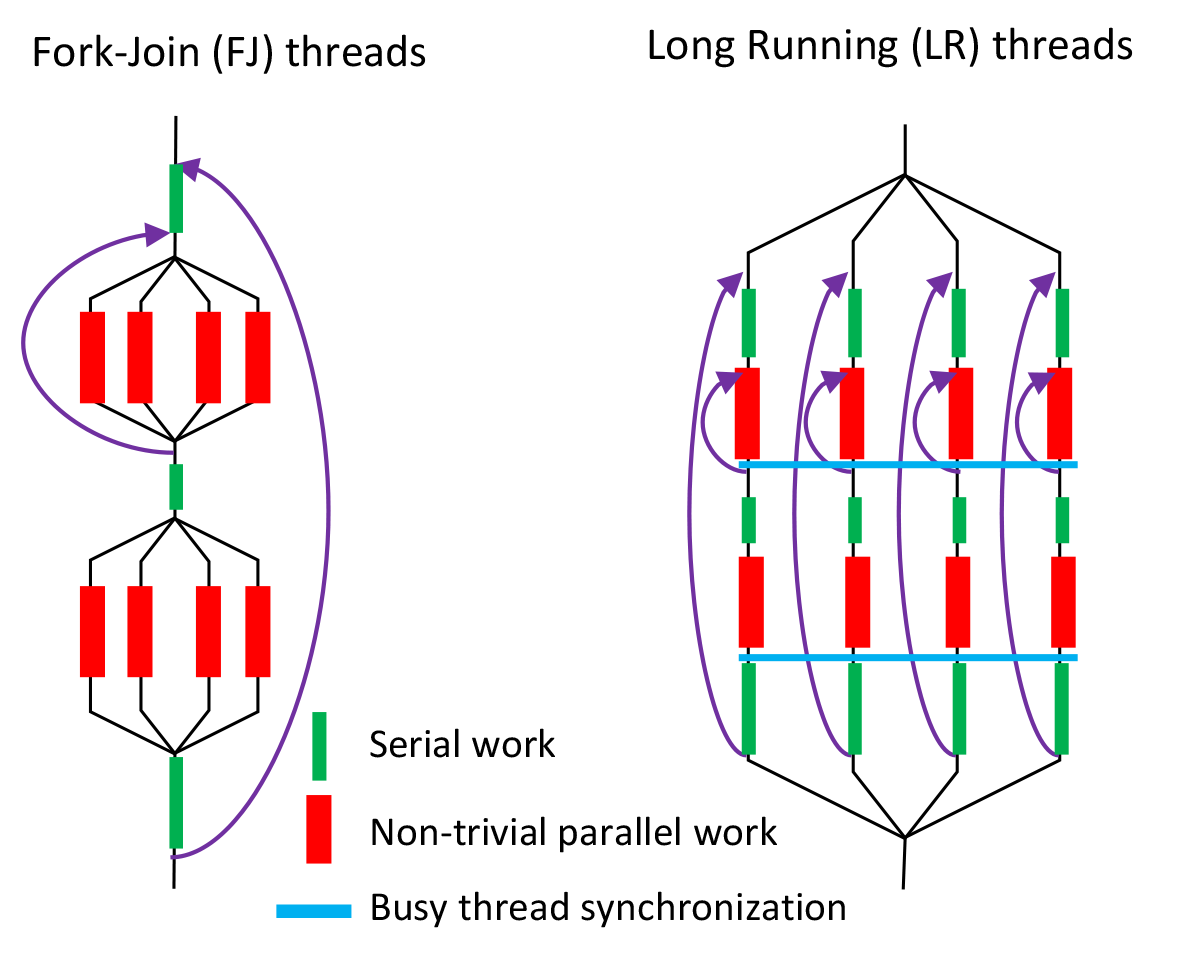
\includegraphics[width=0.6\columnwidth]{images/fig_fj_vs_lrt}
        \caption{Fork-Join vs. long running threads}
        \label{fig:fig_fj_vs_lrt}
    \end{minipage}
    \hspace{1.4mm}
    \begin{minipage}{0.49\textwidth}
        \centering
        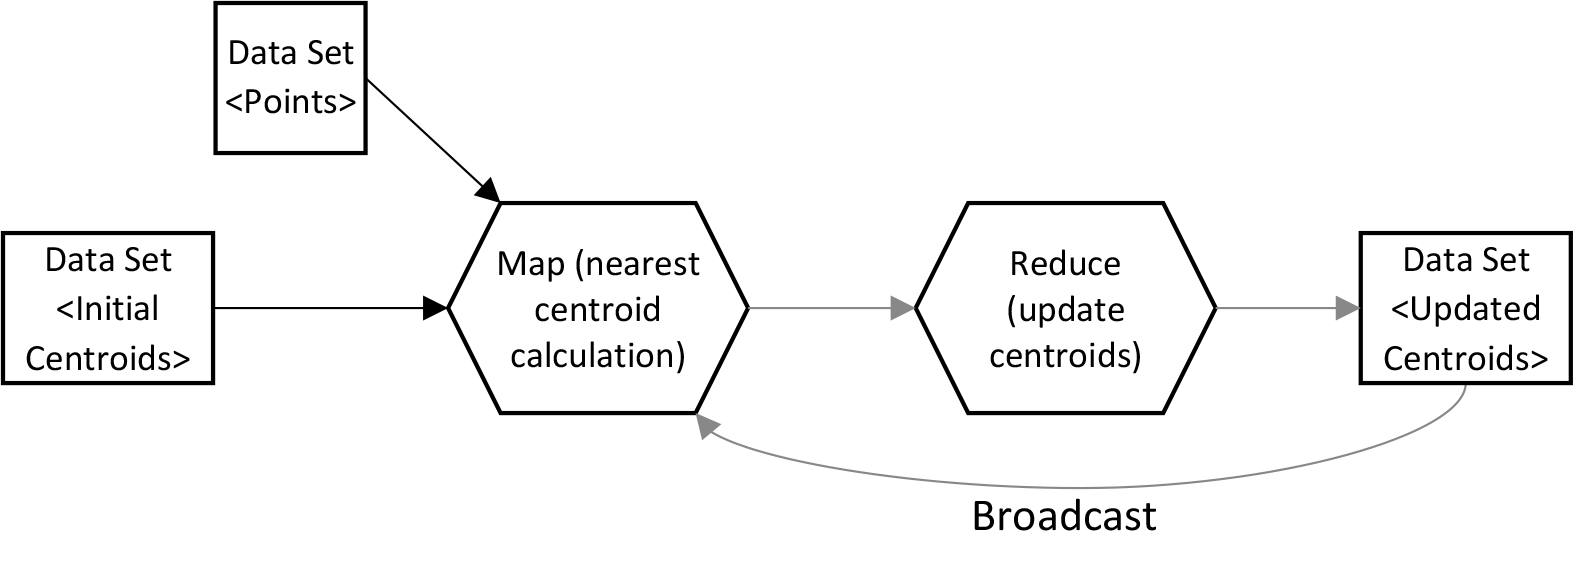
\includegraphics[width=0.9\columnwidth]{images/fig_kmeans_dataflow}
        \caption{Flink k-means algorithm.}
        \label{fig:fig_flink_kmeans}
    \end{minipage}   
\end{figure*}


\section{Evaluation} \label{sec:evaluation}
\textcolor{blue}{TODO - a description of the applications, systems, and results)}

%minipage kmeans Java and C 12 binding patterns
\begin{figure*}[!htb]
    \centering
    \begin{minipage}{.49\textwidth}
        \centering        
        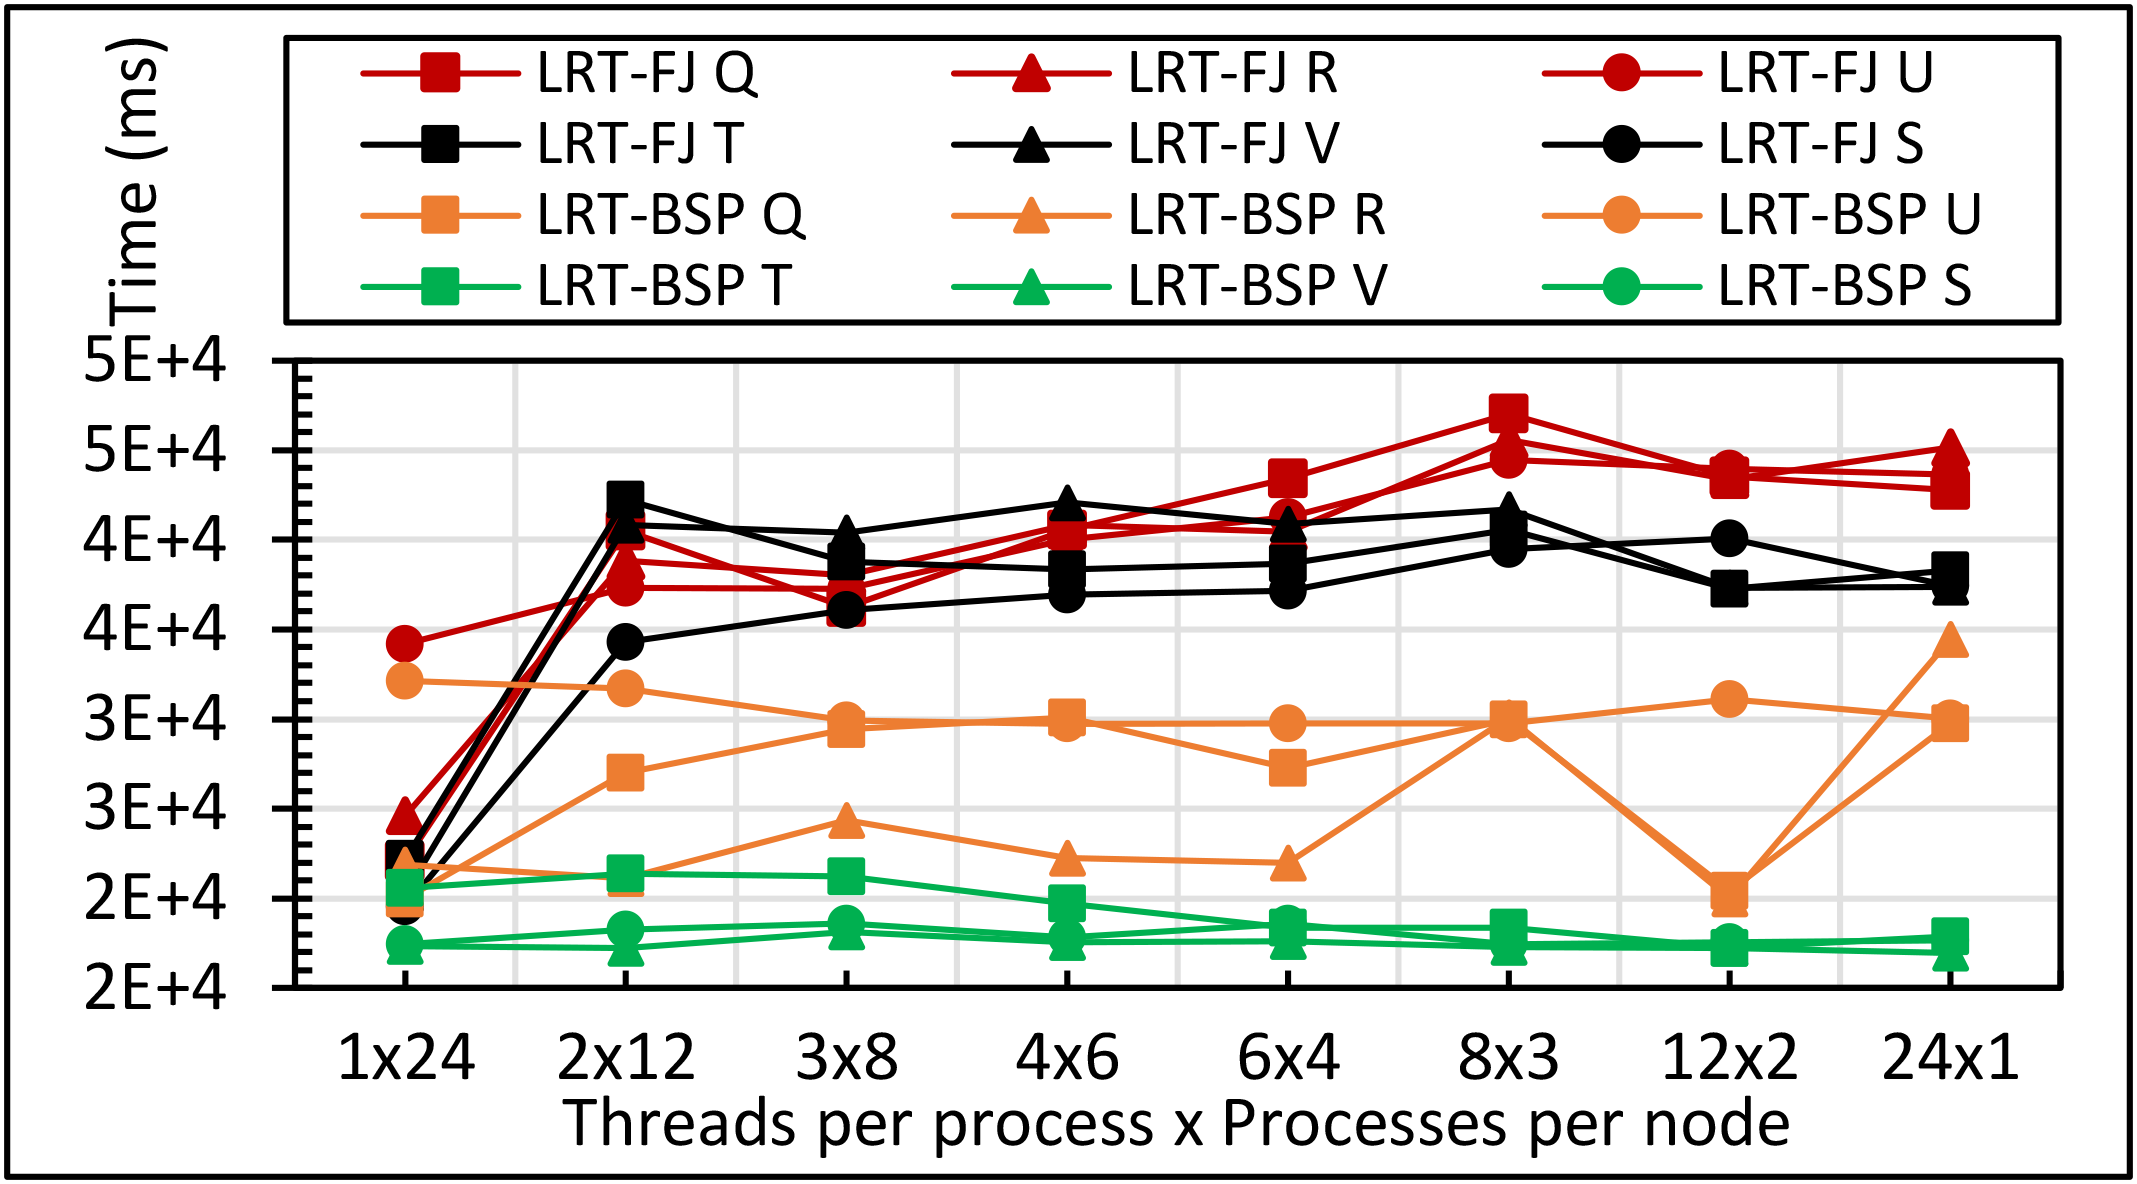
\includegraphics[width=1\columnwidth]{images/fig_kmeans_1mil_1k_binding_patterns}
        \caption{Java k-means 1 mil points and 1k centers performance on 16 nodes for \ac{LRT-FJ} and \ac{LRT-BSP} with varying affinity patterns over varying threads and processes.}
        \label{fig:fig_kmeans_1mil_1k_binding_patterns}
    \end{minipage}
    \hspace{1.4mm}
    \begin{minipage}{0.49\textwidth}
        \centering
        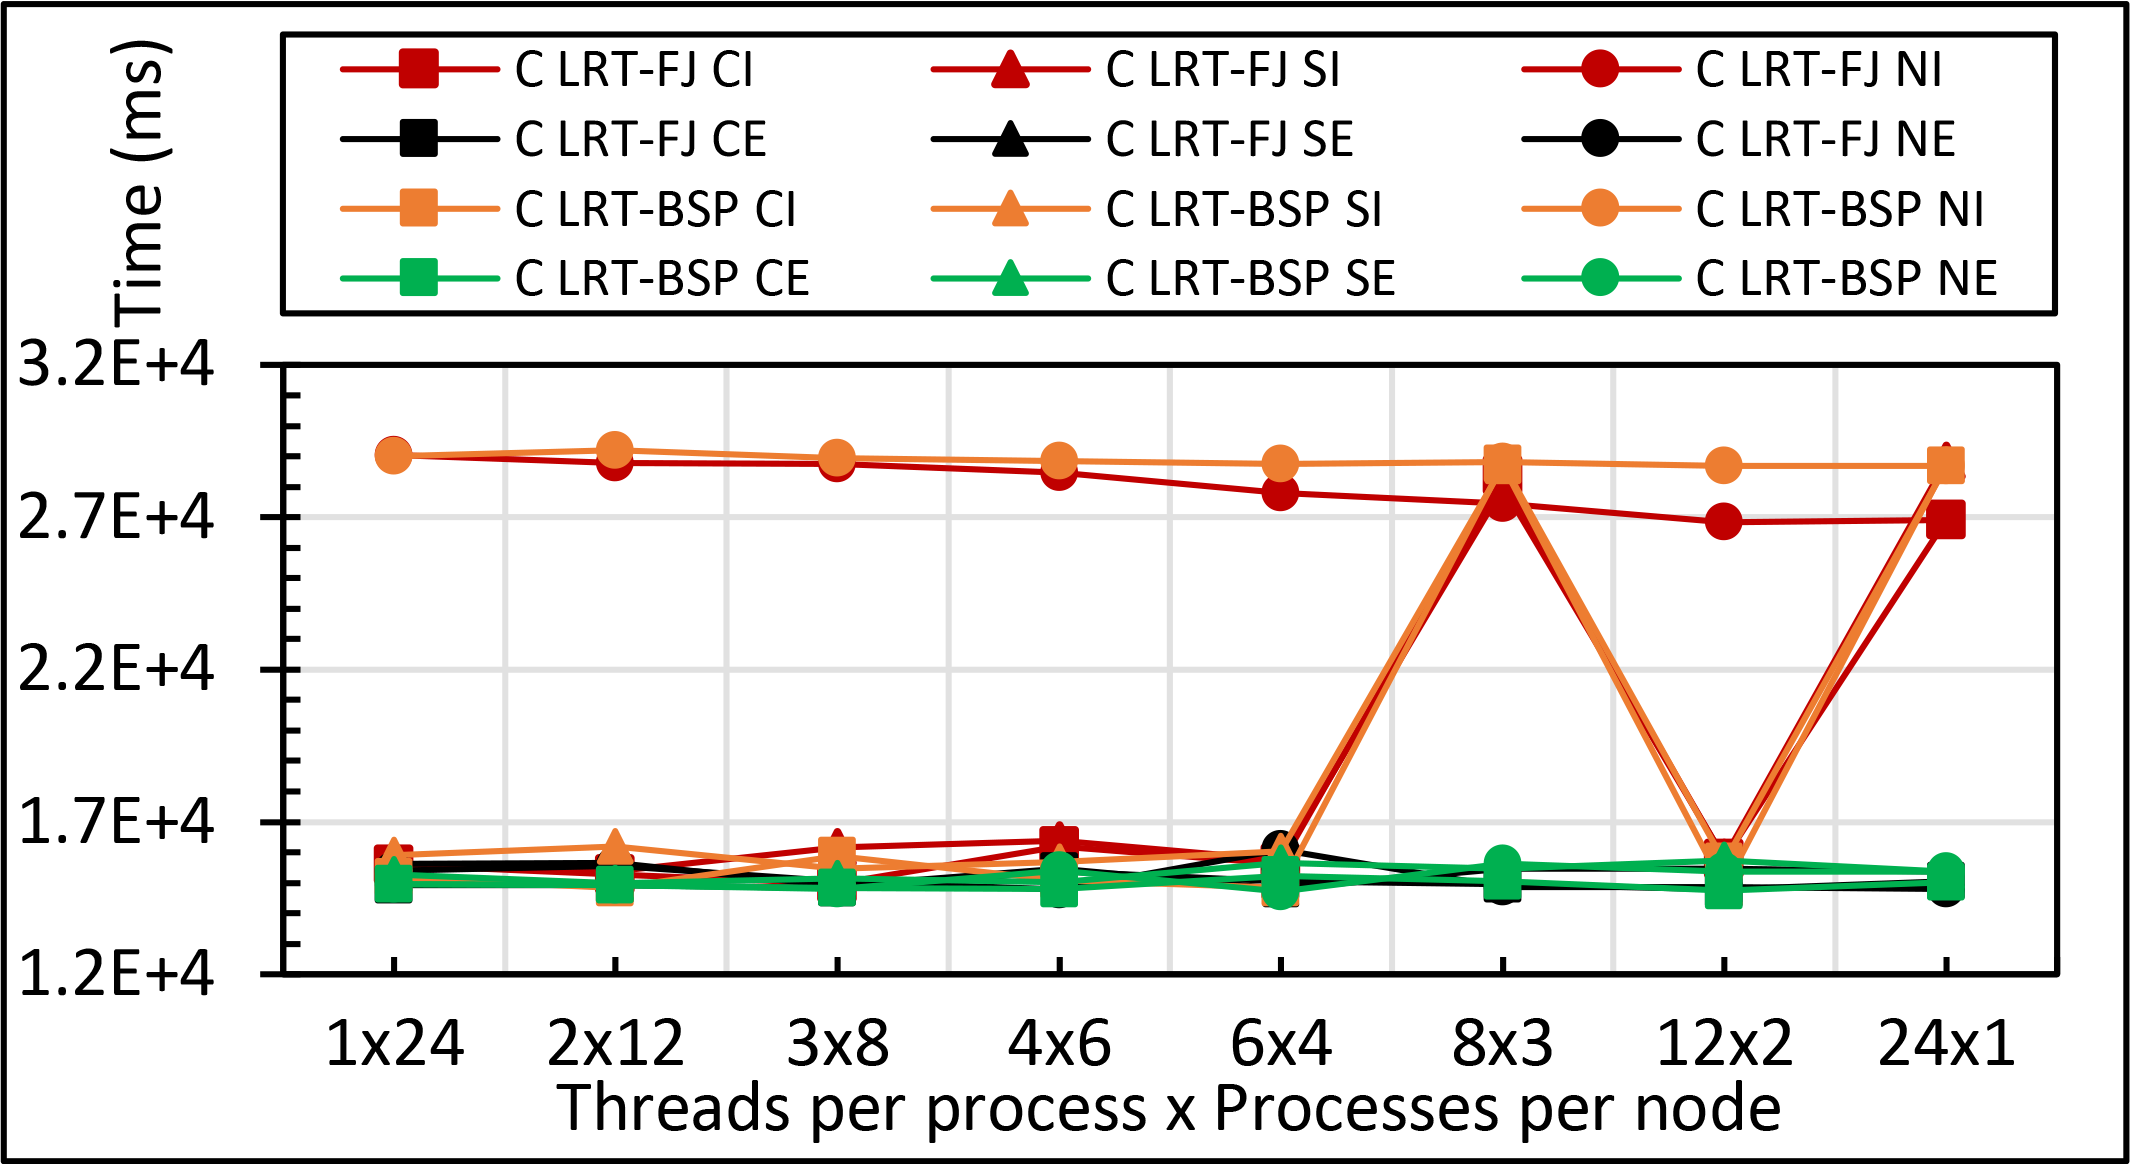
\includegraphics[width=1\columnwidth]{images/fig_C_kmeans_1mil_1k_binding_patterns}
        \caption{C k-means 1 mil points and 1k centers performance on 16 nodes for \ac{LRT-FJ} and \ac{LRT-BSP} with varying affinity patterns over varying threads and processes.}
        \label{fig:fig_C_kmeans_1mil_1k_binding_patterns}
    \end{minipage}   
\end{figure*}

%minipage kmeans Java T vs S | Java vs C
\begin{figure*}[!htb]
    \begin{minipage}{0.49\textwidth}
        \centering
        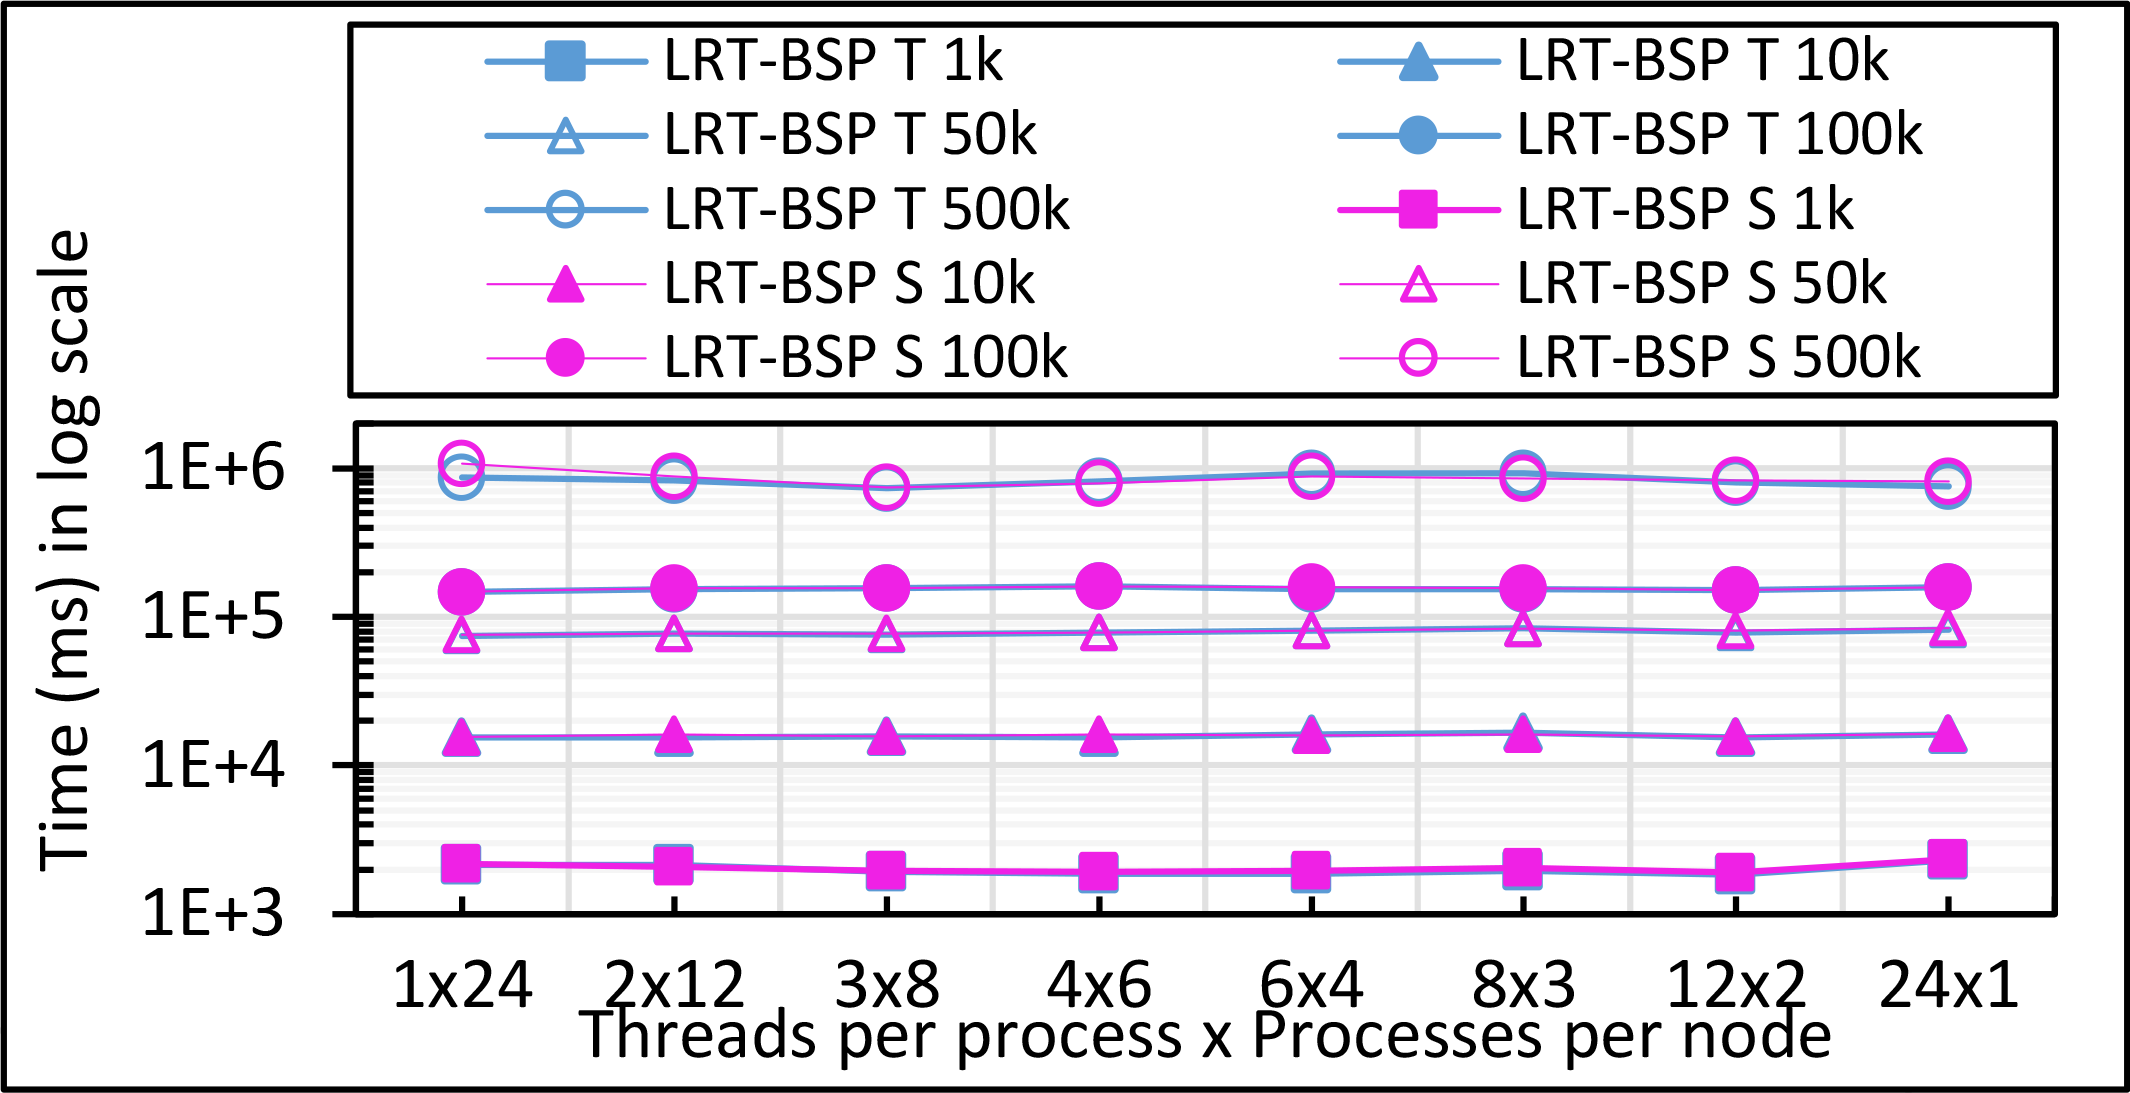
\includegraphics[width=1\columnwidth]{images/fig_kmeans_1mil_varying_centers_BSP_T_vs_BSP_S_Java}
		\caption{Java k-means \ac{LRT-BSP} affinity T vs S performance for 1 mil points with 1k,10k,50k,100k, and 500k centers on 16 nodes over varying threads and processes.}
		\label{fig:images/fig_kmeans_1mil_varying_centers_BSP_T_C_vs_Java}
    \end{minipage}
    \hspace{1.4mm}
    \begin{minipage}{0.49\textwidth}
        \centering
        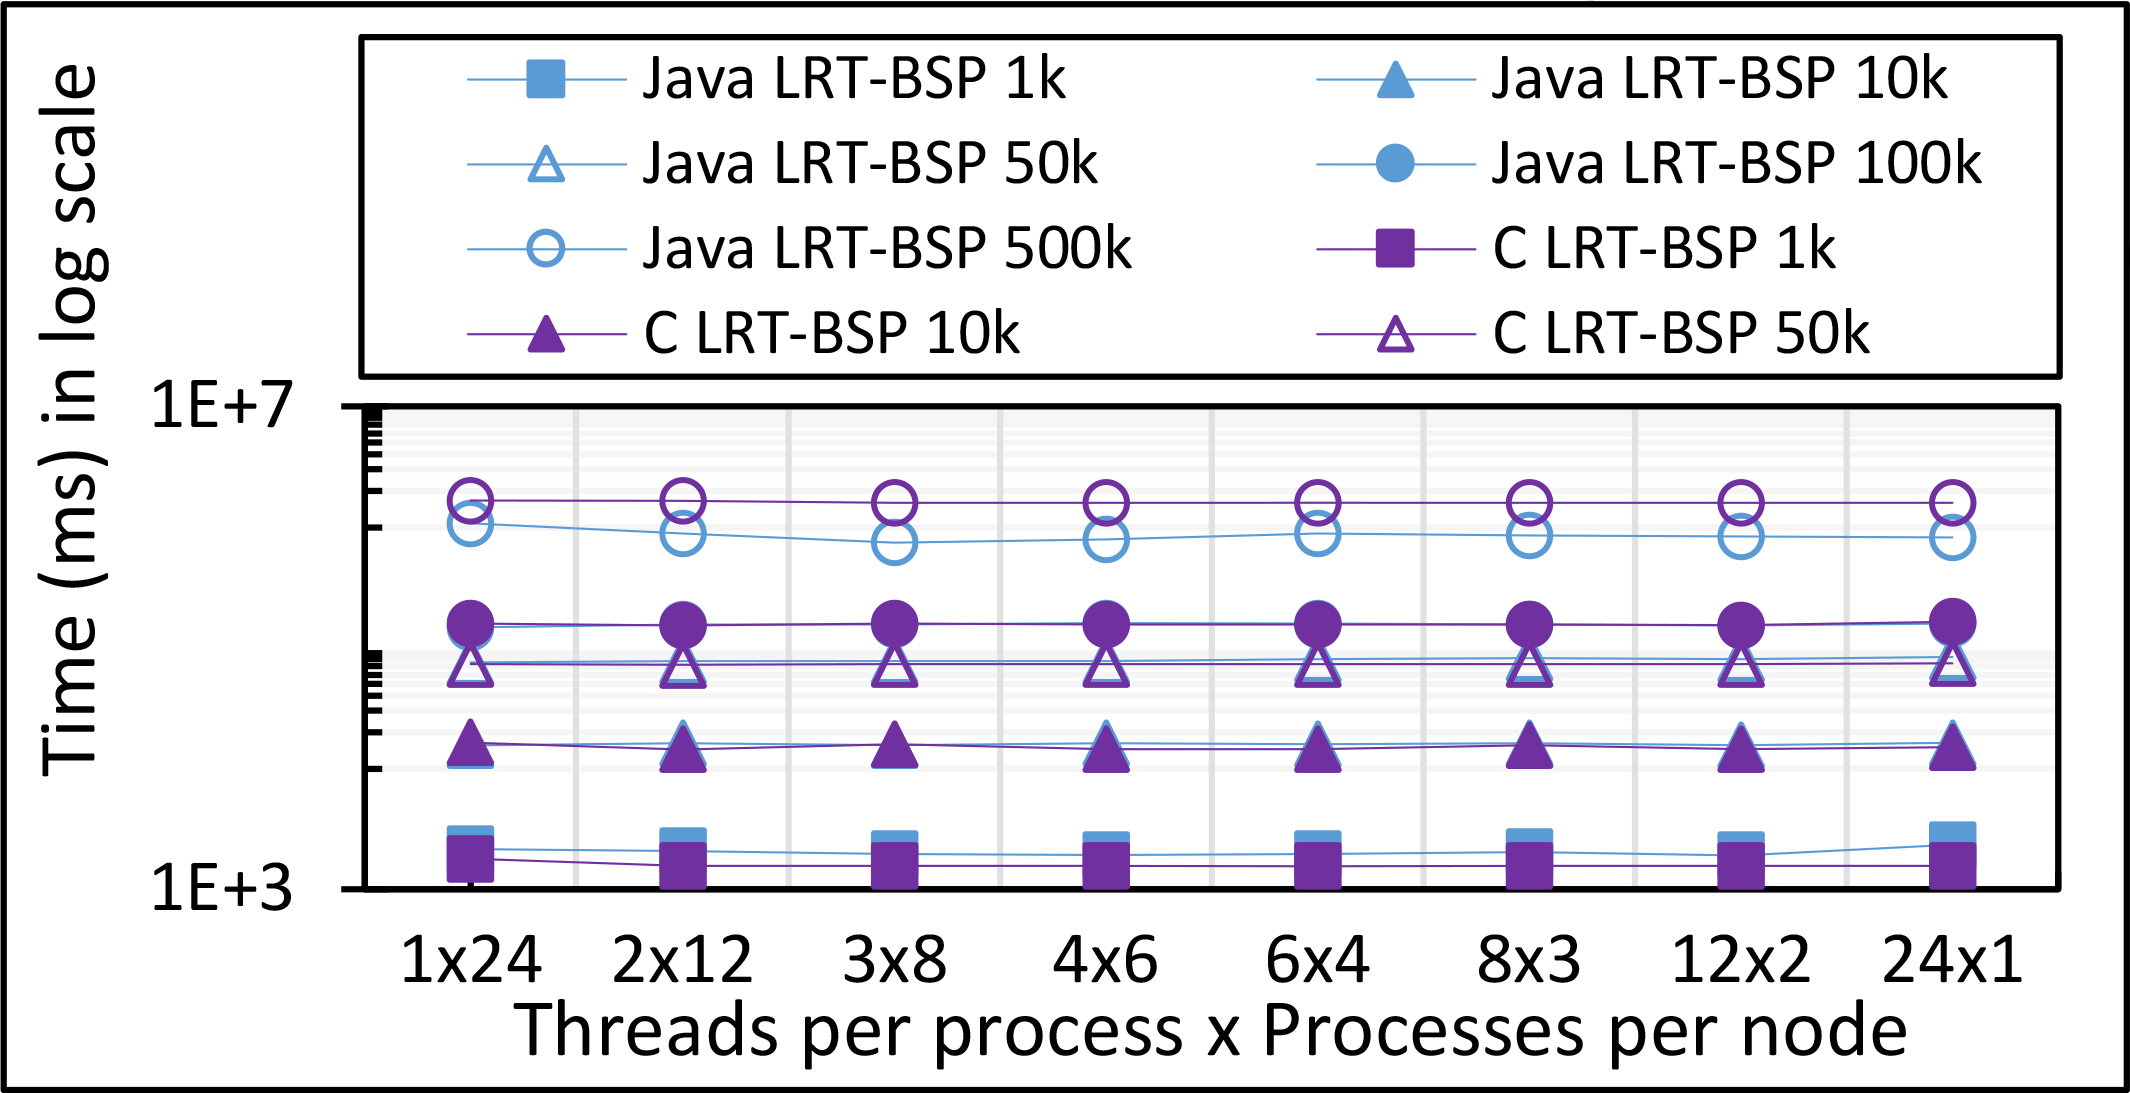
\includegraphics[width=1\columnwidth]{images/fig_kmeans_1mil_varying_centers_BSP_T_C_vs_Java}
		\caption{Java vs C k-means \ac{LRT-BSP} affinity T performance for 1 mil points with 1k,10k,50k,100k, and 500k centers on 16 nodes over varying threads and processes.}
		\label{fig:images/fig_kmeans_1mil_varying_centers_BSP_T_C_vs_Java}
    \end{minipage}   
\end{figure*}

%minipage kmeans 1k,10k,100k | 50k 500k 
\begin{figure*}[!htb]
	\begin{minipage}{0.49\textwidth}
        \centering
        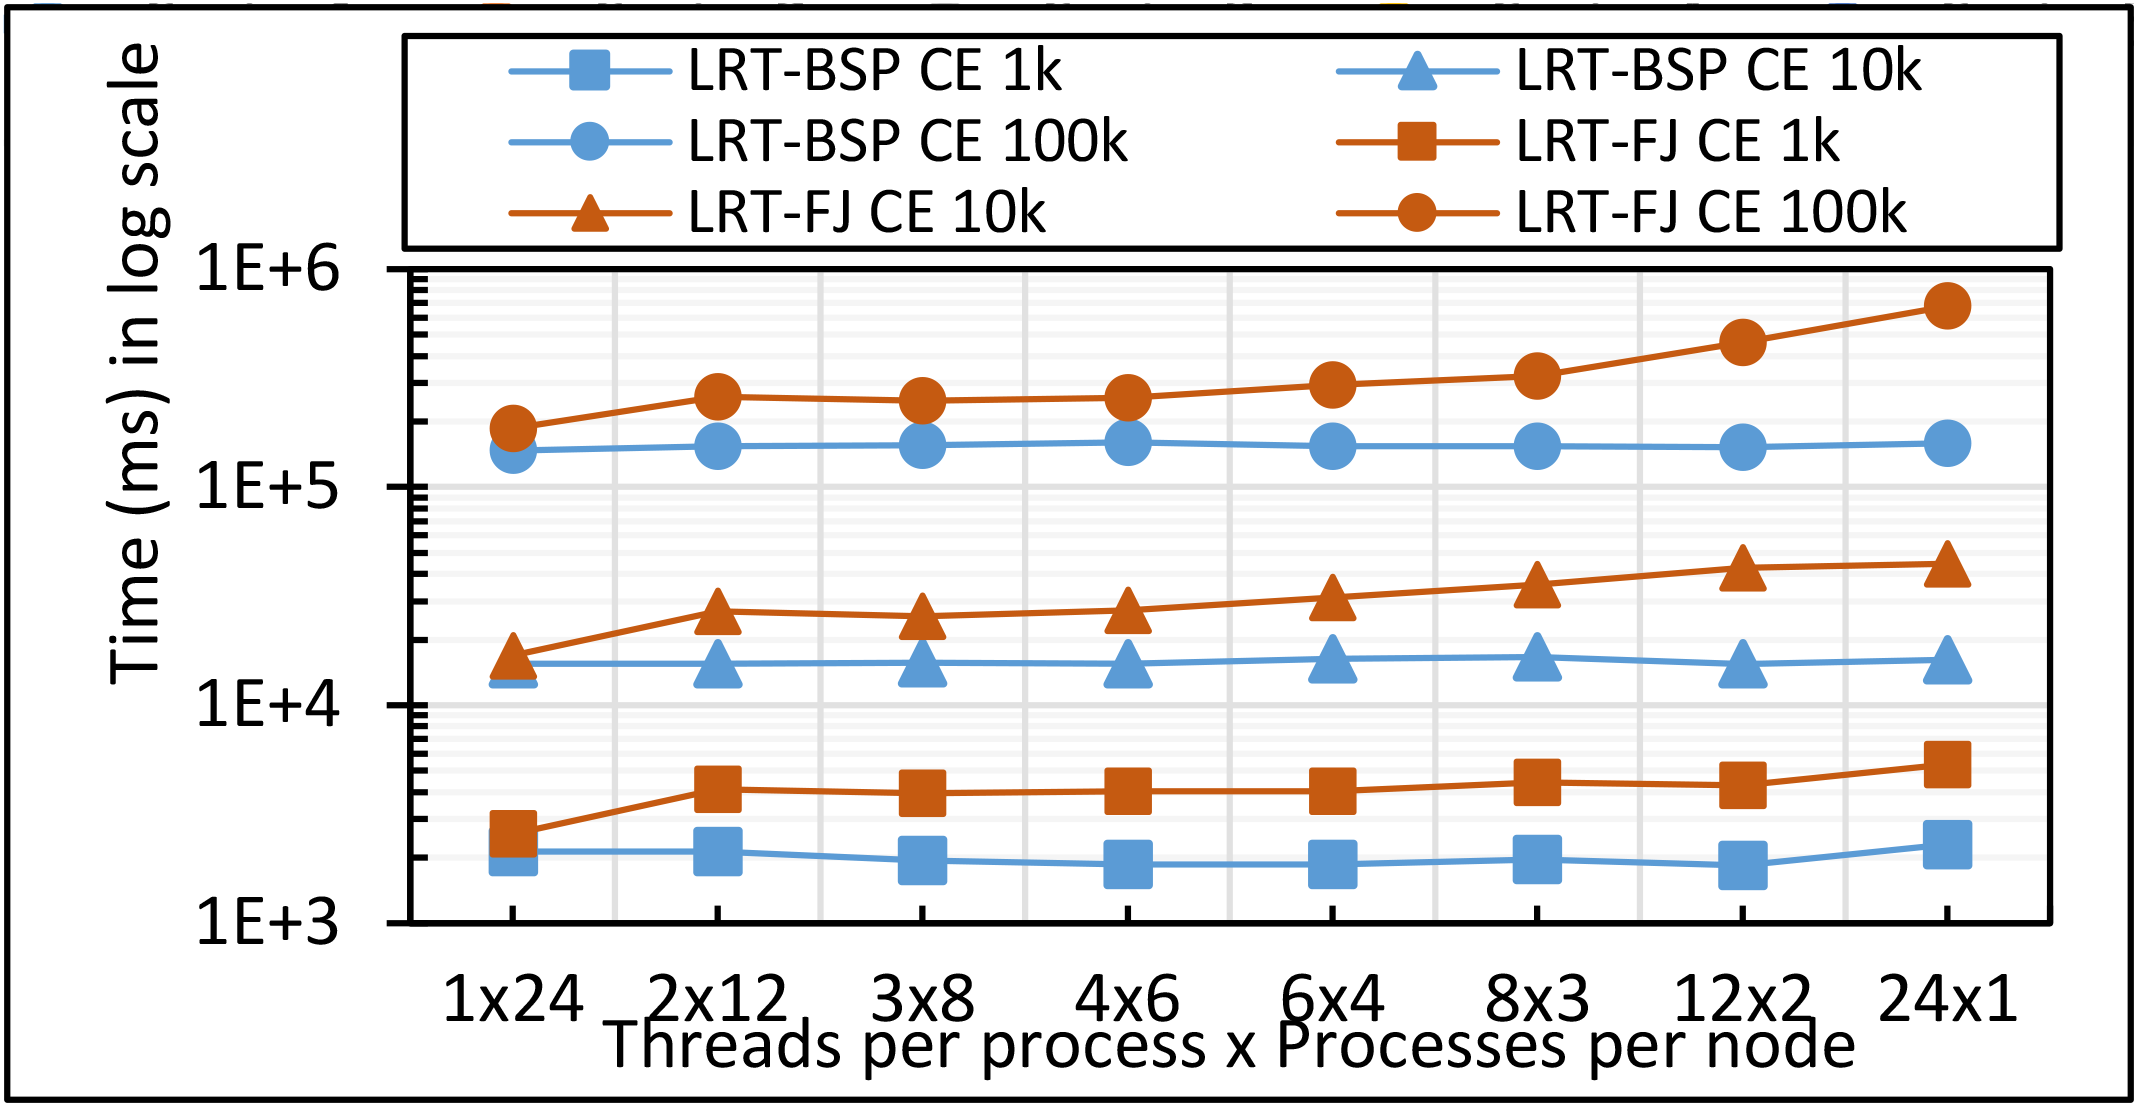
\includegraphics[width=1\columnwidth]{images/fig_kmeans_1mil_varying_centers_by_10k_FJ_vs_BSP_T}
        \caption{Java k-means 1 mil points with 1k,10k, and 100k centers performance on 16 nodes for \ac{LRT-FJ} and \ac{LRT-BSP} over varying threads and processes. The affinity pattern is T.}
        \label{fig:fig_kmeans_1mil_varying_centers_by_10k_FJ_vs_BSP_T}
    \end{minipage}
    \hspace{1.4mm}
    \begin{minipage}{0.49\textwidth}
        \centering
        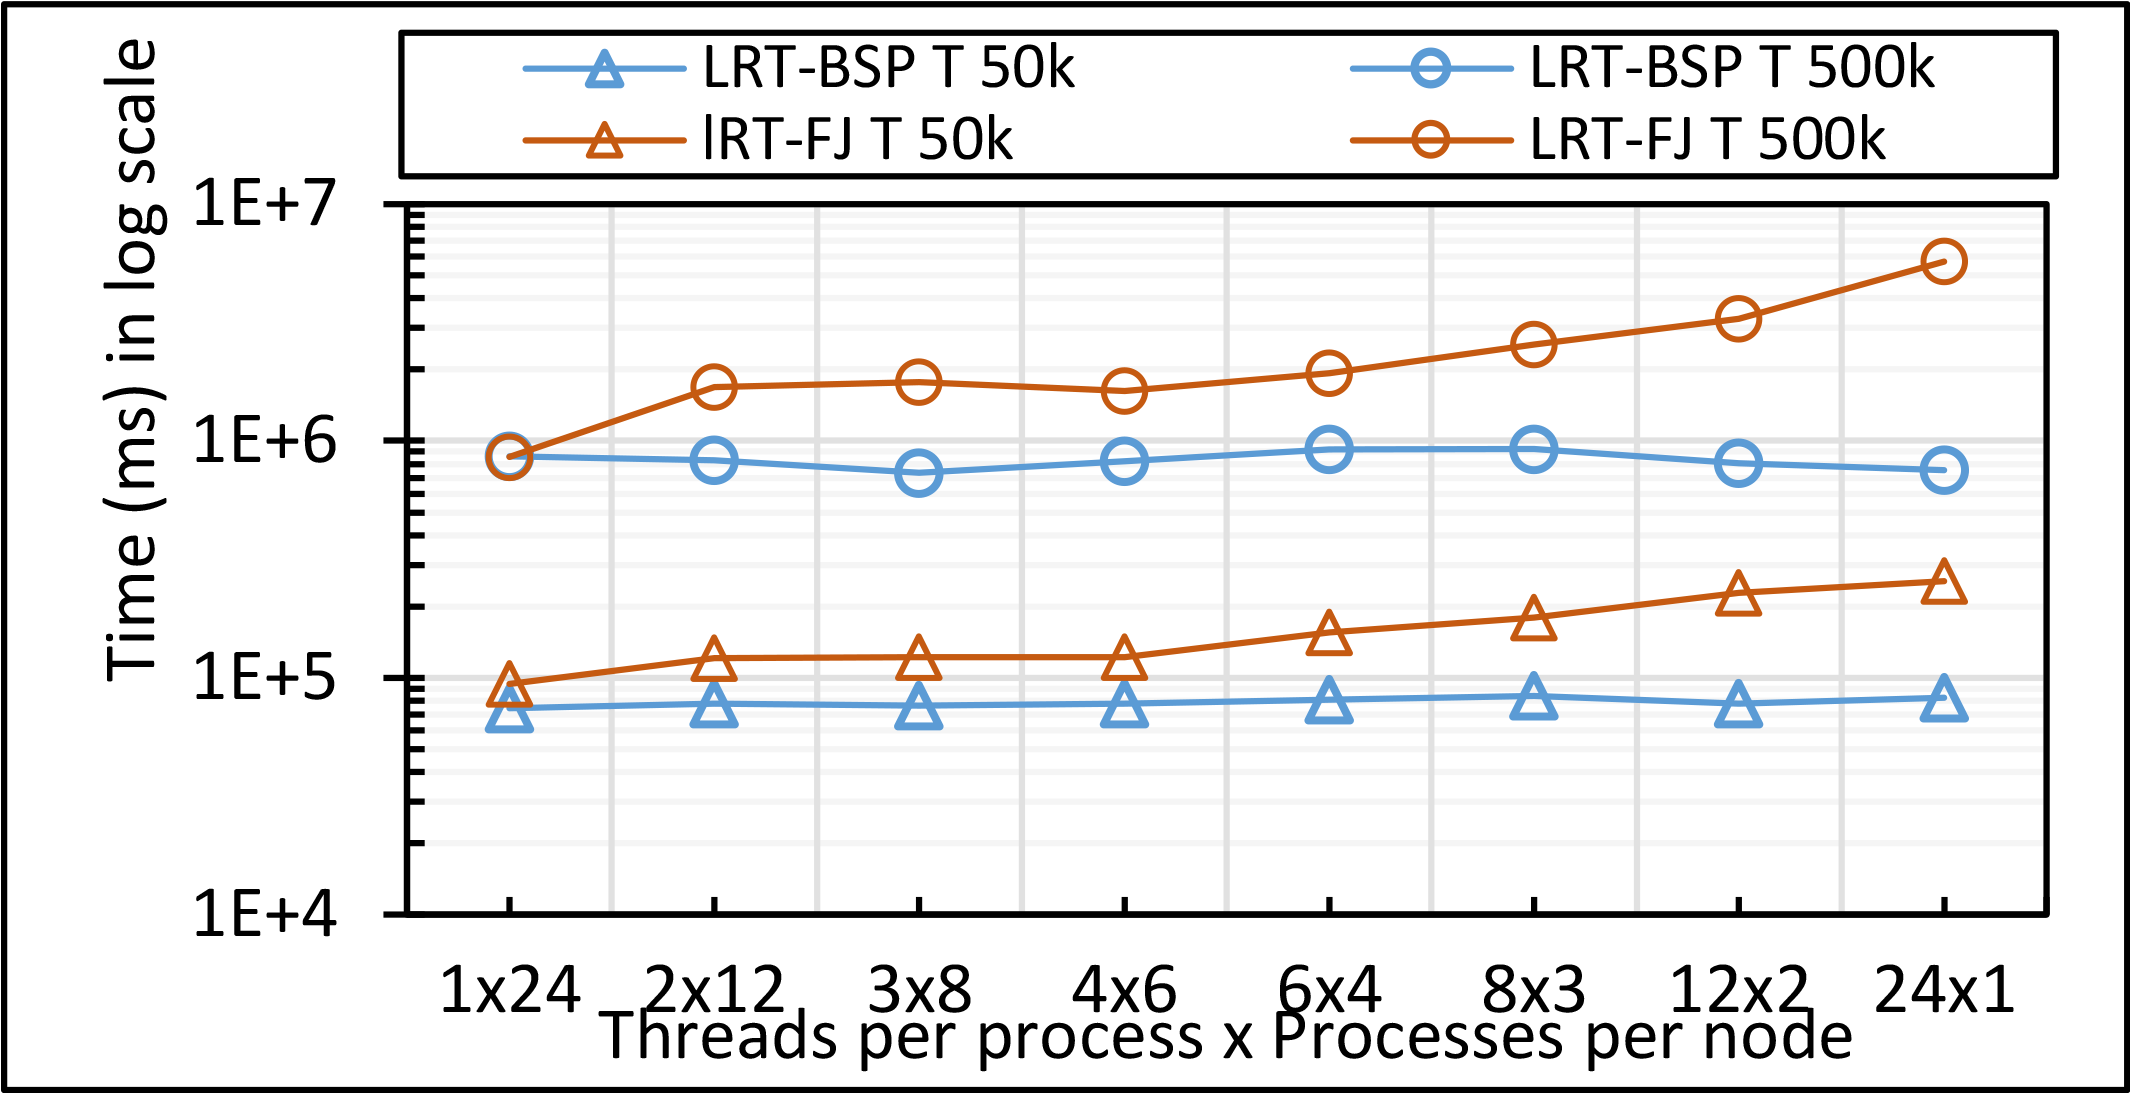
\includegraphics[width=1\columnwidth]{images/fig_kmeans_1mil_varying_centers_as_50k_500k_FJ_vs_BSP_T}
        \caption{Java k-means 1 mil points with 50k, and 500k centers performance on 16 nodes for \ac{LRT-FJ} and \ac{LRT-BSP} over varying threads and processes. The affinity pattern is T.}
        \label{fig:fig_kmeans_1mil_varying_centers_as_50k_500k_FJ_vs_BSP_T}
    \end{minipage}
\end{figure*}

%minipage damds 50k 24core and 36core
\begin{figure*}[!htb]
	\begin{minipage}{0.49\textwidth}
        \centering
        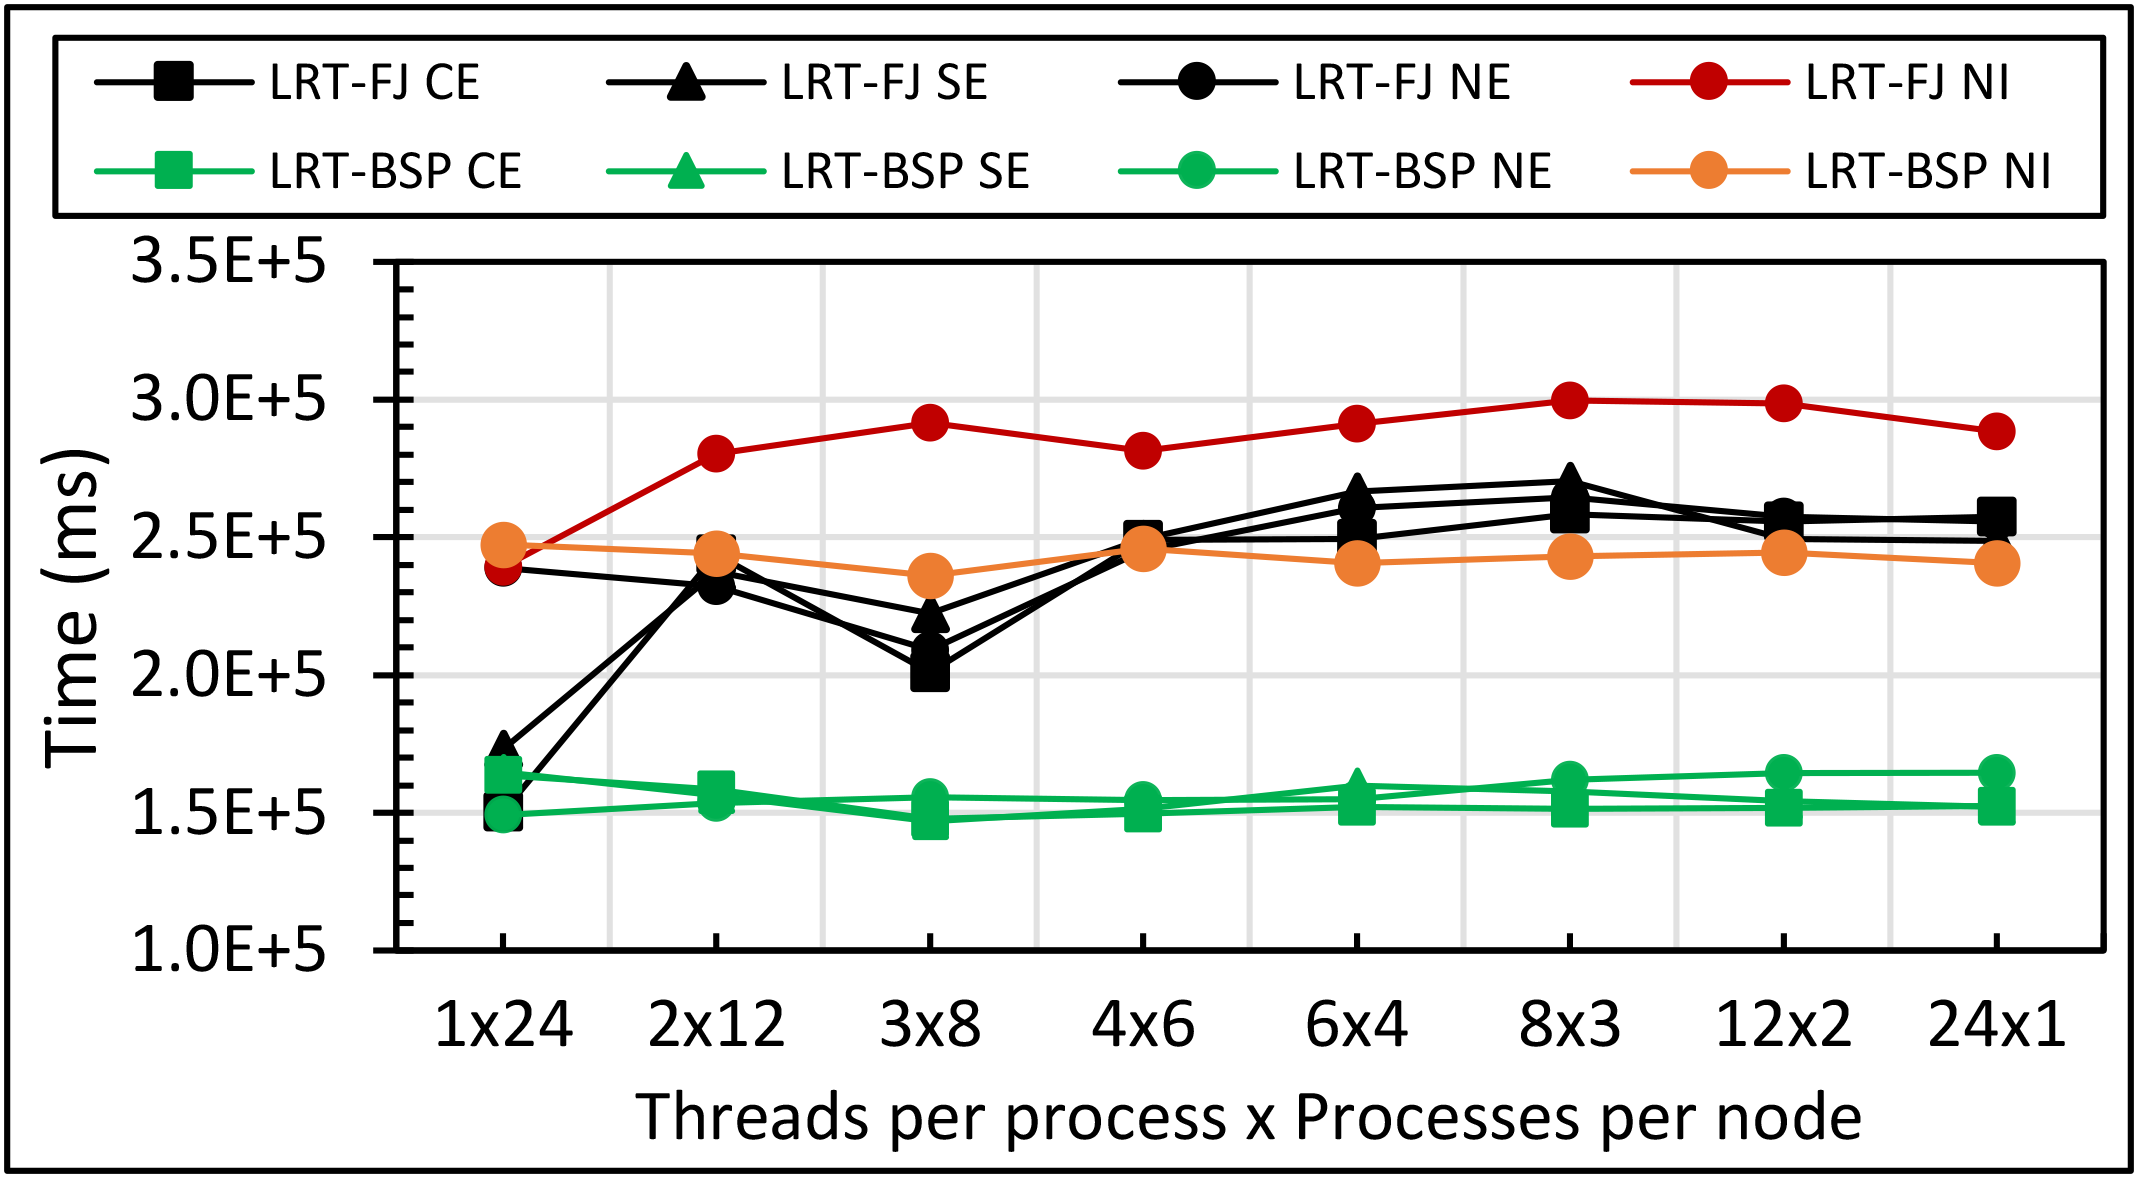
\includegraphics[width=1\columnwidth]{images/fig_damds_50k_binding_patterns}
        \caption{Java DA-MDS 50k points performance on 16 nodes for \ac{LRT-FJ} and \ac{LRT-BSP} over varying threads and processes. Affinity patterns are T,S,V, and U.}
        \label{fig:fig_damds_50k_binding_patterns}
    \end{minipage}
    \hspace{1.4mm}
    \begin{minipage}{0.49\textwidth}
        \centering
        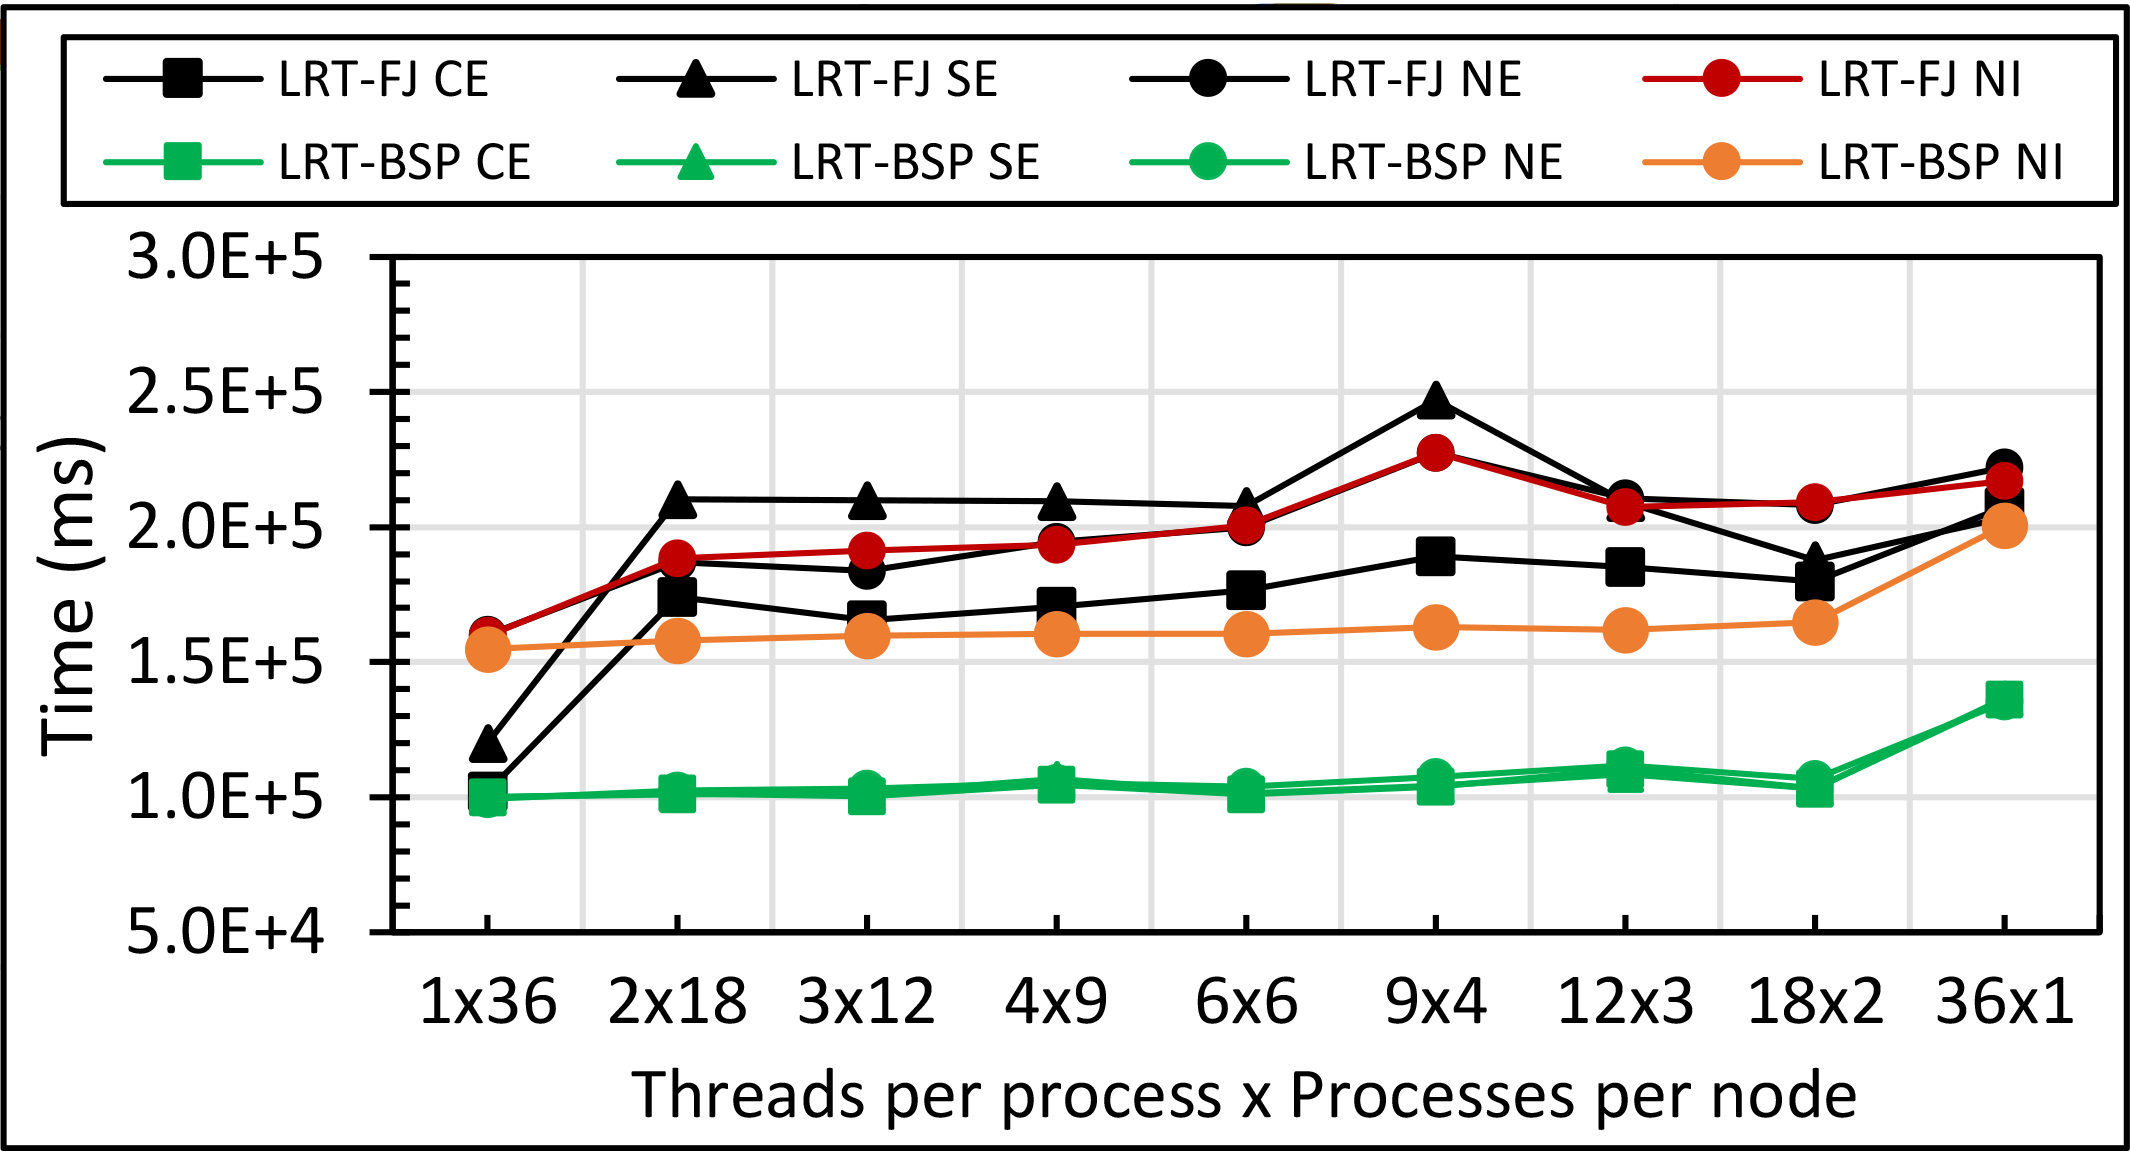
\includegraphics[width=1\columnwidth]{images/fig_damds_50k_binding_patterns_on_36core_nodes}
        \caption{Java DA-MDS 50k points performance on 16 of 36-core nodes for \ac{LRT-FJ} and \ac{LRT-BSP} over varying threads and processes. Affinity patterns are T,S,V, and U.}
        \label{fig:fig_damds_50k_binding_patterns_on_36core_nodes}
    \end{minipage}
\end{figure*}

%minipage damds 100k 24core and 36core
\begin{figure*}[!htb]
	\begin{minipage}{0.49\textwidth}
        \centering
        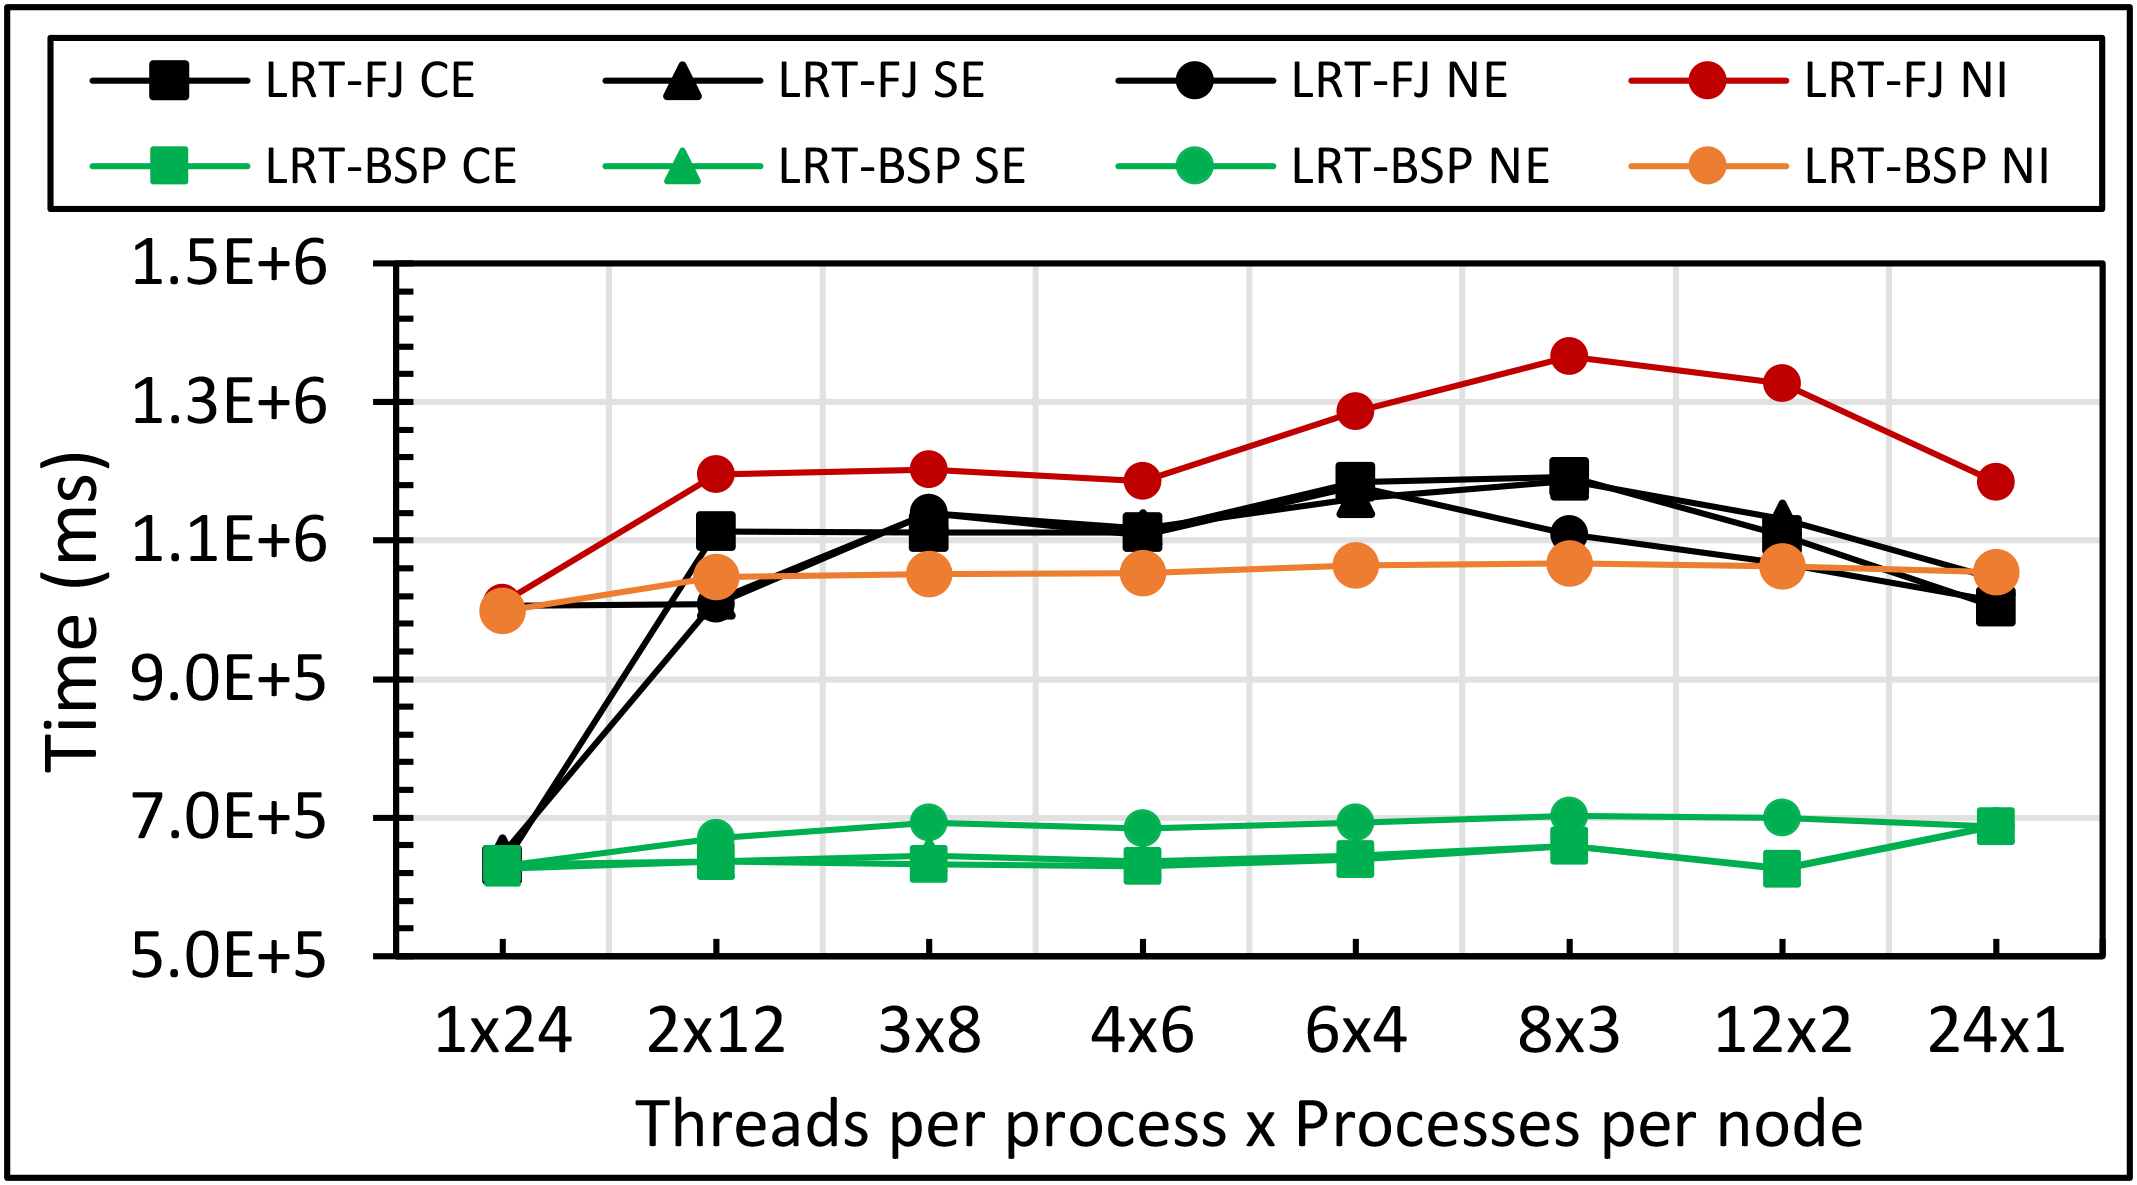
\includegraphics[width=1\columnwidth]{images/fig_damds_100k_binding_patterns}
        \caption{Java DA-MDS 100k points performance on 16 nodes for \ac{LRT-FJ} and \ac{LRT-BSP} over varying threads and processes. Affinity patterns are T,S,V, and U.}
        \label{fig:fig_damds_100k_binding_patterns}
    \end{minipage}
    \hspace{1.4mm}
    \begin{minipage}{0.49\textwidth}
        \centering
        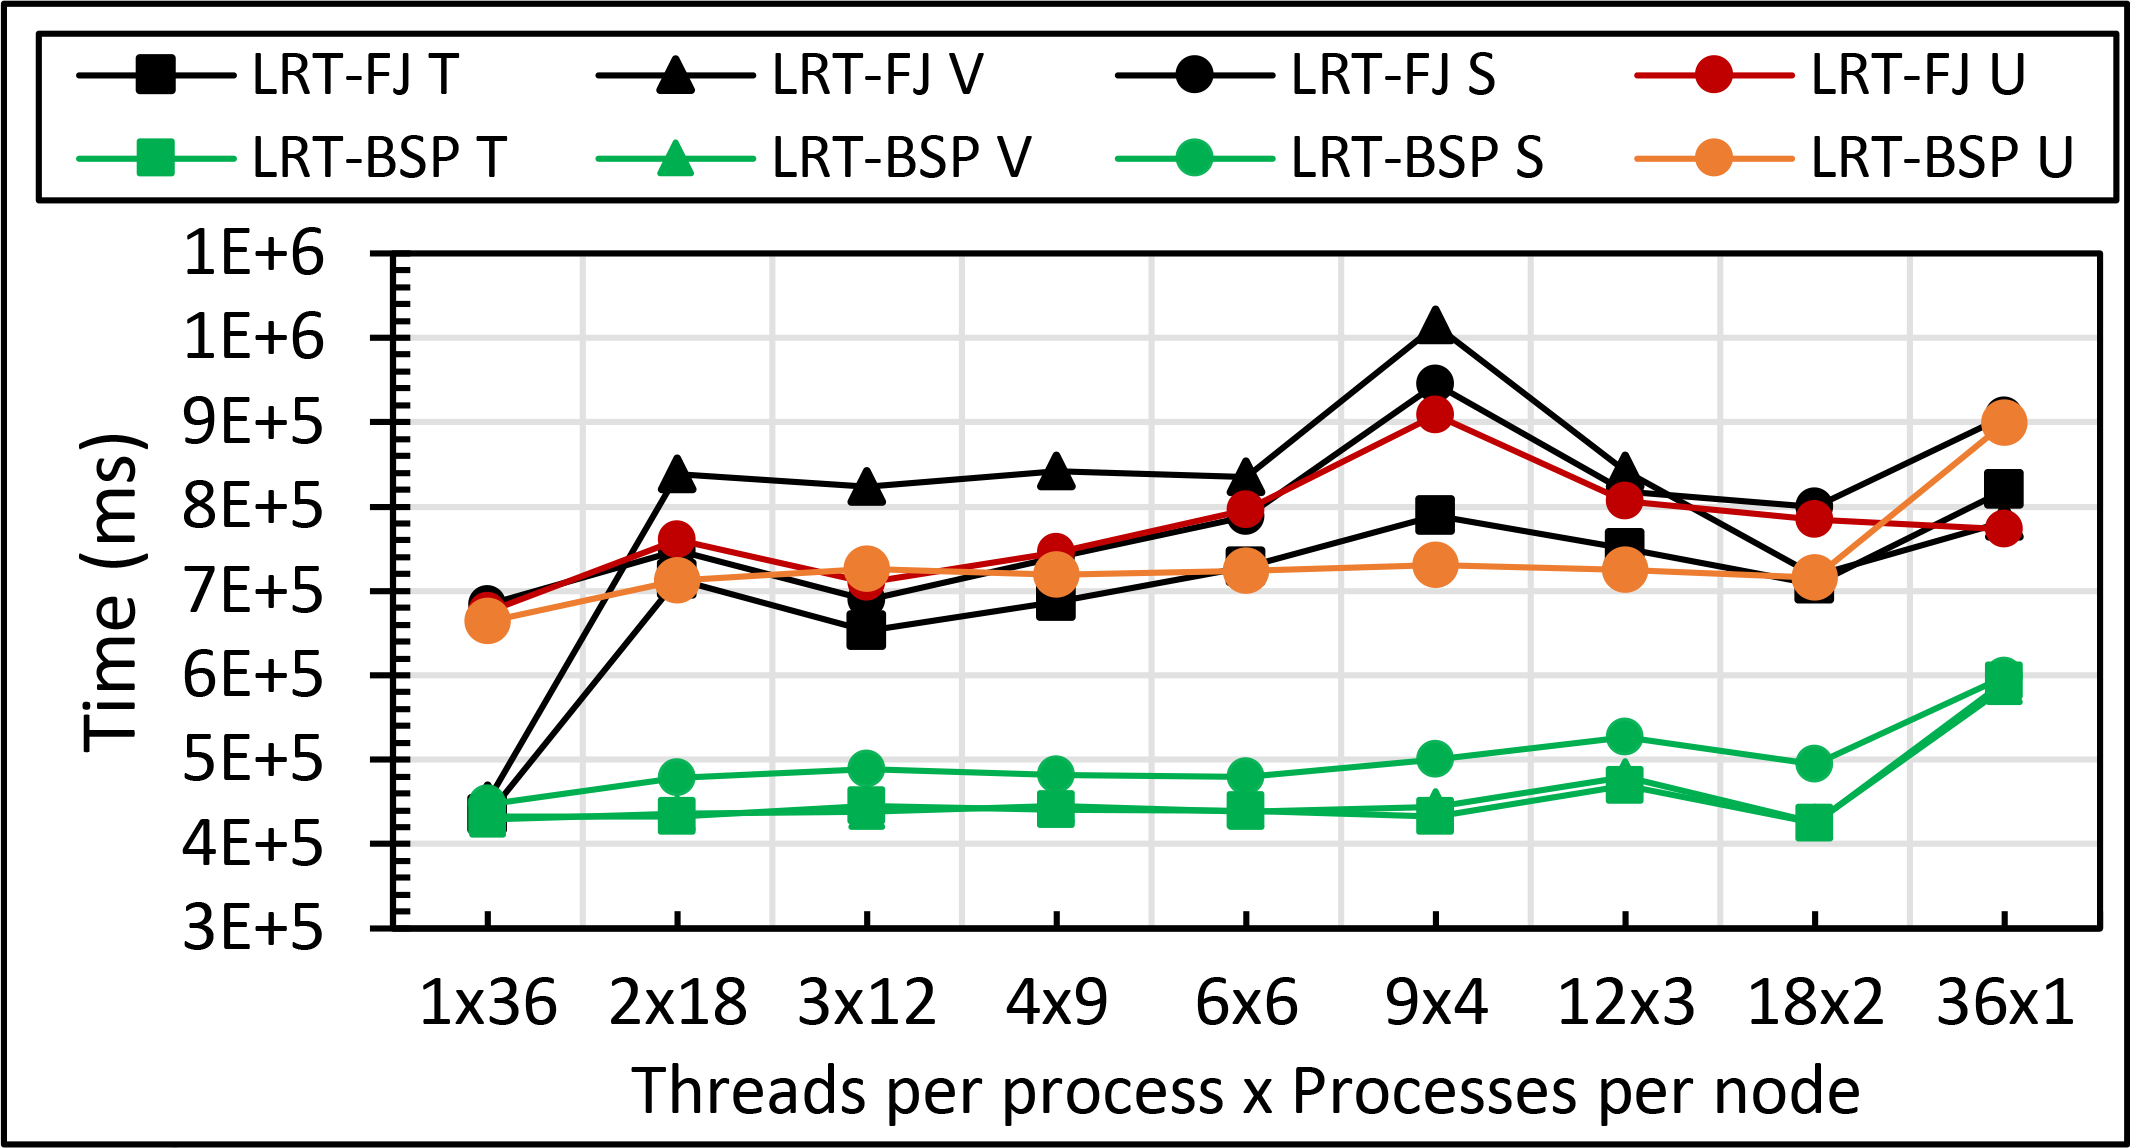
\includegraphics[width=1\columnwidth]{images/fig_damds_100k_binding_patterns_on_36core_nodes}
        \caption{Java DA-MDS 100k points performance on 16 of 36-core nodes for \ac{LRT-FJ} and \ac{LRT-BSP} over varying threads and processes. Affinity patterns are T,S,V, and U.}
        \label{fig:fig_damds_100k_binding_patterns_on_36core_nodes}
    \end{minipage}
\end{figure*}

%minipage damds 200k 24core and 36core
\begin{figure*}[!htb]
	\begin{minipage}{0.49\textwidth}
        \centering
        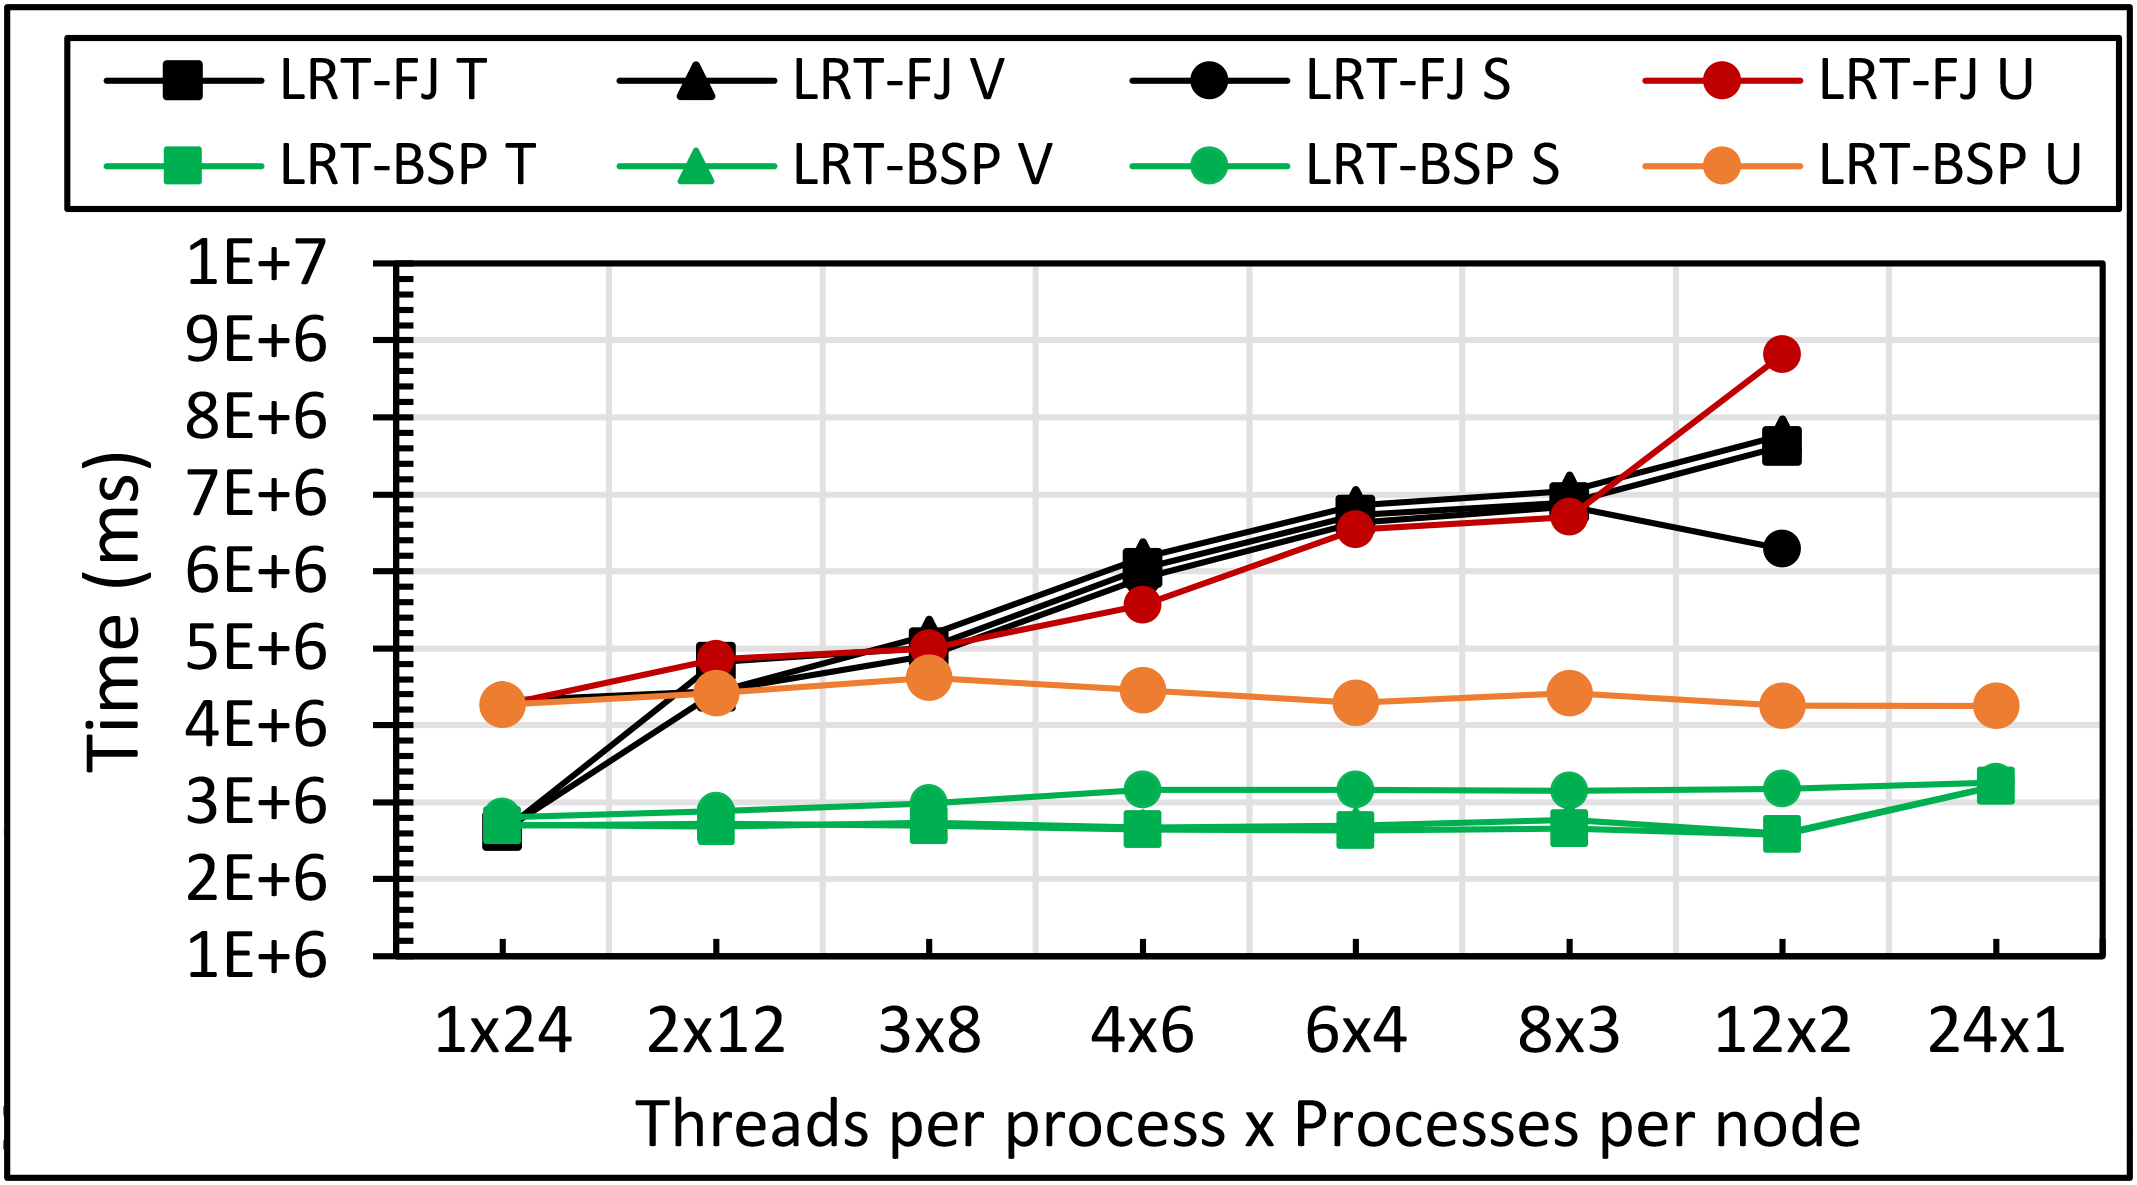
\includegraphics[width=1\columnwidth]{images/fig_damds_200k_binding_patterns}
        \caption{Java DA-MDS 200k points performance on 16 nodes for \ac{LRT-FJ} and \ac{LRT-BSP} over varying threads and processes. Affinity patterns are T,S,V, and U.}
        \label{fig:fig_damds_200k_binding_patterns}
    \end{minipage}
    \hspace{1.4mm}
    \begin{minipage}{0.49\textwidth}
        \centering
        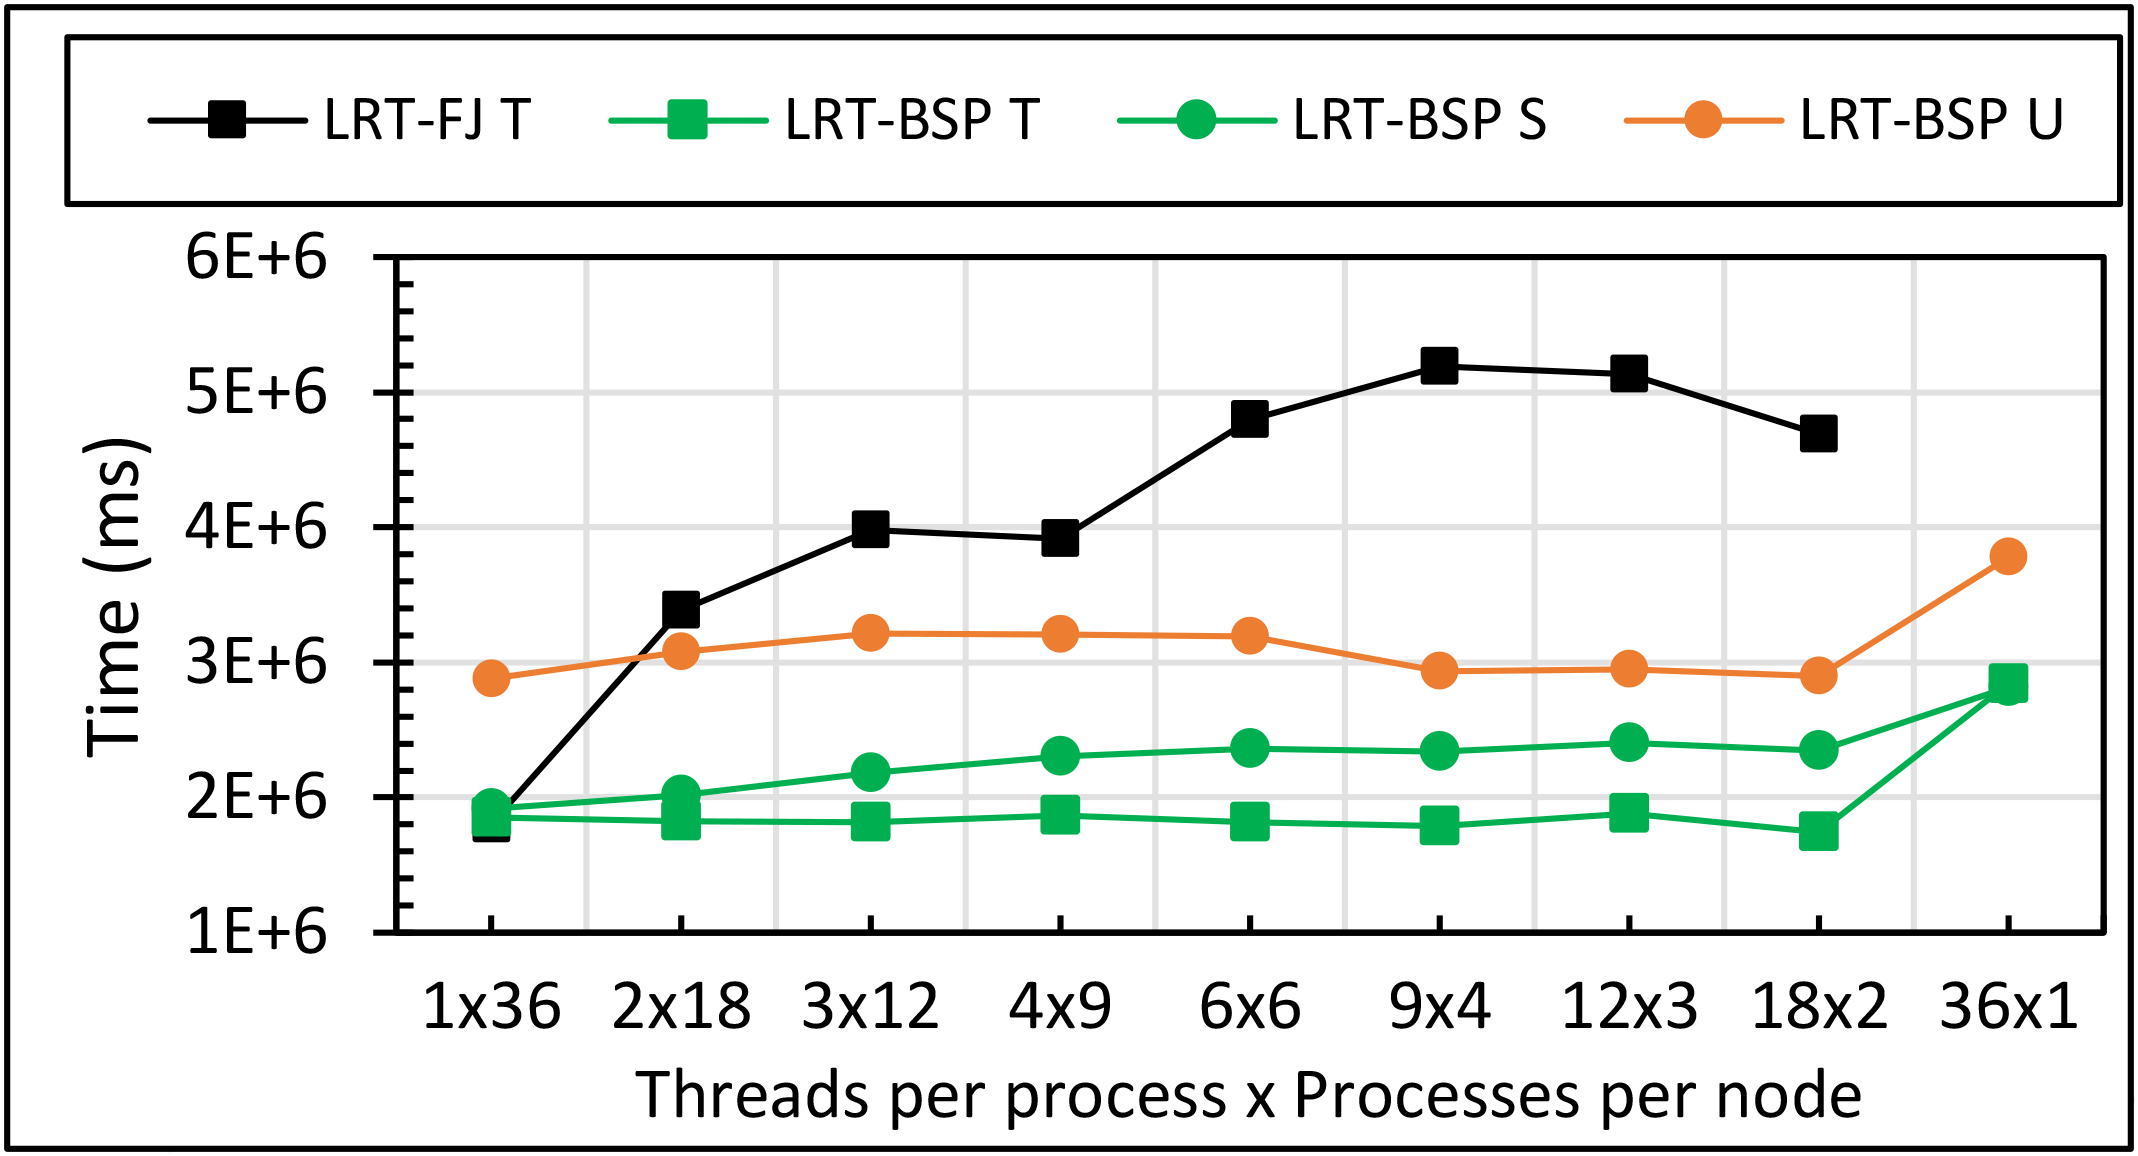
\includegraphics[width=1\columnwidth]{images/fig_damds_200k_binding_patterns_on_36core_nodes}
        \caption{Java DA-MDS 200k points performance on 16 of 36-core nodes for \ac{LRT-FJ} and \ac{LRT-BSP} over varying threads and processes. Affinity patterns are T,S,V, and U.}
        \label{fig:fig_damds_200k_binding_patterns_on_36core_nodes}
    \end{minipage}
\end{figure*}


The experiments were run on Juliet, which is an Intel Haswell \ac{HPC} cluster with 128 nodes total. In this cluster 96 nodes have 24 cores (2 sockets x 12 cores each) and 32 nodes have 36 cores (2 sockets x 18 cores each) per node. Each node consists of 128GB of main memory and 56Gbps Infiniband interconnect and 1Gbps dedicated Ethernet connections. \ac{MPI} runs used the Infiniband except when comparing against Flink and Spark, where all three frameworks used \ac{TCP} communications.

\subsection{MPI Java and C K-Means}
\figurename~\ref{fig:fig_kmeans_1mil_1k_binding_patterns} and \figurename~\ref{fig:fig_C_kmeans_1mil_1k_binding_patterns} show k-means Java and C total runtime for 1 million 2D points and 1000 centroids respectively. Each figure present performance of both \ac{LRT-FJ} and \ac{LRT-BSP} models over the six binding patterns identified in~\ref{tbl:affinity_patterns}. These were run on 24-core nodes; hence the abscissa shows all the eight possible combinations of threads and processes within a node to exploit the full 24-way parallelism. The left most pattern, 1x24, indicates all processes and the right most pattern, 24x1 indicates all threads within a node. Note, patterns 8x3 and 24x1 span processes across \ac{NUMA} boundaries, which is known to be inefficient but presented here for completeness. The red and orange lines represent inherited thread affinity for \ac{LRT-FJ} and \ac{LRT-BSP} respectively. Similarly, the black and green lines illustrate explicit thread pinning, each to a core, for these two thread models. 

Java results suggest \ac{LRT-FJ} is the worst despite the affinity strategy for any pattern other than 1x24, which is all \ac{MPI} and does not use thread parallel regions. A primary reason for this poor performance is the thread scheduling overhead in Java as \ac{FJ} threads are short-activated. Also, the \ac{JVM} spawns extra bookkeeping threads for \ac{GC} and other tasks, which compete for \acs{CPU} resources as well. Of the \ac{LRT-BSP} lines, the unbound threads (\texttt{U}) shows the worst performance. Affinity patterns \texttt{S} and \texttt{T} seem to give the best runtime with increasing number of threads. 

C results show the same behavior for unbounded and explicitly bound threads. The two thread models, however, show similar performance, unlike Java. Further investigation of this behavior revealed OpenMP threads keep the \acsp{CPU} occupied at 100\% between \ac{FJ} regions suggesting OpenMP internally optimizes threads similar to the Java \ac{LRT-BSP} implementation introduced in this paper.

\figurename~\ref{fig:images/fig_kmeans_1mil_varying_centers_BSP_T_C_vs_Java} illustrates the effect of affinity patterns \texttt{T} and \texttt{S} for varying data sizes on \ac{LRT-BSP}. They performed similar to each other, but numbers favor pattern \texttt{T} over \texttt{S}.

\figurename~\ref{fig:images/fig_kmeans_1mil_varying_centers_BSP_T_C_vs_Java} compares Java and C \ac{LRT-BSP} runtimes for k-means over varying data sizes across thread and process combinations. Results demonstrate Java performance is on par with C. Also, sometimes Java outperform C, mostly due to \ac{JIT} optimizations, as seen in the figure for 500k centers. 

\figurename~\ref{fig:fig_kmeans_1mil_varying_centers_by_10k_FJ_vs_BSP_T} and \figurename~\ref{fig:fig_kmeans_1mil_varying_centers_as_50k_500k_FJ_vs_BSP_T} showcase \ac{LRT-FJ} and \ac{LRT-BSP} performance over varying data sizes for affinity pattern \texttt{T}. In \figurename~\ref{fig:fig_kmeans_1mil_varying_centers_by_10k_FJ_vs_BSP_T}, the number of centroids were incremented as 1k,10k, and 100k. \ac{LRT-BSP} show constant performance across thread and process combinations for all data sizes, where as \ac{LRT-FJ} exhibit abysmal performance with increasing threads and data sizes. \figurename~\ref{fig:fig_kmeans_1mil_varying_centers_as_50k_500k_FJ_vs_BSP_T} replicates the same experiment for data sizes 50k and 500k. Again, the results agree with that of \figurename~\ref{fig:fig_kmeans_1mil_varying_centers_by_10k_FJ_vs_BSP_T}.

\subsection{Flink K-Means}
We evaluated the performance of k-means algorithm with Apache Flink. The evaluation was done in 16 node clusters each with 24 cores. The primary objective of the test was to measure the performance of Flink k-means compared to the MPI version. We also evaluated the computation time versus the total time, which gives an estimate about the other overheads including communication. We observed very high communication overhead compared to the MPI version. This is mainly due to sub-optimal implementation of reduction in Flink.

Since the communication overhead is dominating the distributed execution of k-means algorithm, we conducted an experiment in a single machine with one process to see the overheads of thread execution. With one process there is no network communication in Flink. Flink uses an actor-based execution model with Akka~\cite{gupta2012akka} framework to execute the tasks. The framework creates \ac{LRT-FJ} style threads to execute the individual tasks. With this experiment, we have observed execution time imbalances among the parallel tasks. The same has been observed with the \ac{LRT-FJ} Java MPI implementation of k-means and we could potentially minimize these effects in MPI Java with the \ac{LRT-BSP} style executions. Balanced parallel computations are vital to efficient parallel algorithms as the slowest task dominates the parallel computation time. 

\subsection{Spark K-Means}
Spark k-means was evaluated similar to the Flink implementation on a 16 node cluster with 24 cores on each node. In order to compare its performance against the MPI implementation of k-mean,s we observed total execution times. Additionally in order to understand the effect of other overheads in Spark we observed computation times separately. Similar to what we observed in Flink, the total execution time was dominated by communication overheads in reduce operations and broadcast operations. 
In order to observe thread overheads and other overheads that are involved with task creation and execution in the spark execution model , we ran tests on a single 24 core node. Only a single executor was created that handled 24 tasks. Spark uses an executor/task model where an executor creates at most a single task for each core that is allocated to the executor. As with Flink, we observed that there are imbalances between execution times for parallel tasks. This leads to longer total execution times since the total execution time is dependent on the slowest task. 



%speedup table
\begin{table}[]
\centering
\caption{Java \ac{DA-MDS} speedup for varying data sizes on 24-core and 36-core nodes. Red values indicate the suboptimal performance of \ac{LRT-FJ} model compared to \ac{LRT-BSP}. Ideally, these values should be similar to their immediate left cell values.}
\label{tbl:mds-speedup}
\setlength\tabcolsep{6pt}
\setlength\extrarowheight{4pt}
\begin{tabular}{@{}c@{}|@{}C@{}|@{}C@{}|@{}C@{}|@{}C@{}|@{}C@{}|@{}C@{}|@{}C@{}|@{}C@{}|@{}C@{}|}
\cline{2-10}
                                     & \multicolumn{9}{c|}{\textbf{Data Size}}                                                                                                                                                                                              \\ \cline{2-10} 
\multicolumn{1}{c|}{}                & \multicolumn{3}{c|}{\textbf{50k}}                                          & \multicolumn{3}{c|}{\textbf{100k}}                                         & \multicolumn{3}{c|}{\textbf{200k}}                                         \\ \hline
\multicolumn{1}{|c|}{\textbf{Nodes}} & \textbf{1x24 LRT-BSP} & \textbf{12x2 LRT-BSP} & \textbf{12x2 LRT-FJ}       & \textbf{1x24 LRT-BSP} & \textbf{12x2 LRT-BSP} & \textbf{12x2 LRT-FJ}       & \textbf{1x24 LRT-BSP} & \textbf{12x2 LRT-BSP} & \textbf{12x2 LRT-FJ}       \\ \hline
\multicolumn{1}{|c|}{16}             & 1                     & 1                     & {\color[HTML]{FE0000} 0.6} & 1                     & 1                     & {\color[HTML]{FE0000} 0.6} & 1                     & 1                     & {\color[HTML]{FE0000} 0.4} \\ \hline
\multicolumn{1}{|c|}{32}             & 2.2                   & 2                     & {\color[HTML]{FE0000} 1.1} & 1.9                   & 1.9                   & {\color[HTML]{FE0000} 1.1} & 1.9                   & 2                     & {\color[HTML]{FE0000} 0.6} \\ \hline
\multicolumn{1}{|c|}{64}             & 3.9                   & 3.6                   & {\color[HTML]{FE0000} 1.9} & 3.6                   & 3.6                   & {\color[HTML]{FE0000} 1.9} & 3.7                   & 3.8                   & {\color[HTML]{FE0000} 0.9} \\ \hline
\multicolumn{1}{|c|}{\textbf{Nodes}} & \textbf{1x36 LRT-BSP} & \textbf{18x2 LRT-BSP} & \textbf{18x2 LRT-FJ}       & \textbf{1x36 LRT-BSP} & \textbf{18x2 LRT-BSP} & \textbf{18x2 LRT-FJ}       & \textbf{1x36 LRT-BSP} & \textbf{18x2 LRT-BSP} & \textbf{18x2 LRT-FJ}       \\ \hline
\multicolumn{1}{|c|}{16}             & 1                     & 1                     & {\color[HTML]{FE0000} 0.6} & 1                     & 1                     & {\color[HTML]{FE0000} 0.6} & 1                     & 1.1                   & {\color[HTML]{FE0000} 0.4} \\ \hline
\multicolumn{1}{|c|}{32}             & 2                     & 1.8                   & {\color[HTML]{FE0000} 0.9} & 1.9                   & 1.9                   & {\color[HTML]{FE0000} 1.1} & 1.9                   & 2.1                   & {\color[HTML]{FE0000} 0.6} \\ \hline
\end{tabular}
\end{table}

\section{Discussion}
Spark and Flink are widely used efficient big data platforms for processing large amounts of data as well as executing machine learning algorithms. Both are in-memory computation platforms, unlike Hadoop which is primarily a disk-based platform. These systems are designed to handle large amounts of data and be fault tolerant in case of failures. They can use disks as an auxiliary storage if the data is too large to fit in the memory. 

On the other hand, MPI is a lightweight framework with excellent communication and execution semantics that are  well suited for high performance multi-core clusters. We believe Java MPI implementations, along with the careful design of executions and communications in multi-core clusters discussed in this work, provide a performance ceiling for Java-based machine learning applications. This study shows many factors that are critical for achieving the best possible performance and scalability and how they can be carefully tuned. 

Current implementations of the big data computation frameworks lack the efficient communication algorithms implemented in MPI platforms. With current implementations of Spark and Flink, we have identified efficient communication as the most potentially detrimental feature in getting to the best possible performance. 

The computation time variations in the parallel tasks of Flink and Spark frameworks can be attributed to the \ac{LRT-FJ} style invocations and Garbage collection. It is hard to completely avoid the GC overheads, but Flink-like systems have adopted off-heap memory management for reducing the effect. The \ac{LRT-BSP} style threads can  help in reducing the compute time variations, as evident by the MPI Java applications.  


\section{Related Work} \label{sec:related}
There are libraries such as MPI implementations available for Java; Guillermo et al.~\cite{taboada2013java} discusses their performance in HPC environments. In our work we use OpenMPI Java bindings because our preliminary studies showed it performed the best among the available options. MPJ-Express~\cite{baker2006mpj} and JaMP~\cite{klemm2007jamp} are popular pure Java implementation of the MPI standard. Rajesh et al.~\cite{karmani2009actor} discusses actor-based frameworks to exploit the multi-core machines and Flink uses actor model for handling concurrency. Maria et al.~\cite{carpen2015performance} show how to optimize the Java Garbage collection in multi-core NUMA machines.

Much research has been done on how to get better performance on multi-core clusters using hybrid execution model of threads and processes~\cite{chorley2010performance, rabenseifner2009hybrid, camp2011streamline}. They discuss the performance across NUMA sockets, as well as how threads and processes perform in conjunction. In this work we apply these techniques in the context of machine learning algorithms to get scalable performance.

Recent work by the authors~\cite{kamburugamuve2016towards} have improved communications of Apache Storm streaming framework with classical collective algorithms found in MPI implementations. Harp~\cite{zhang2015harp} is a collective communication framework developed for Hadoop to speed up the machine learning applications. Previous work by authors~\cite{hpc2016:spidaljava} focused on improving the collective communications for machine learning algorithms using shared memory for intra-node messaging.

\section{Conclusion} \label{sec:conclusion \& Future Work}
In this paper we discussed how to obtain consistent scalable performance of machine learning algorithms implemented in Java in large multi-core clusters. The deficiencies in performance we observed before the improvements in Java MPI machine learning applications can be observed on the current implementations of big data run-times such as Flink and Spark, and we are working on bringing these improvements to such frameworks.


% use section* for acknowledgement
\section*{Acknowledgment}
This work was partially supported by NSF CIF21 DIBBS 1443054 and NSF RaPyDLI 1415459. We thank Intel  for their support of the Juliet system, and extend our gratitude to the FutureSystems team for their support with the infrastructure. 

% trigger a \newpage just before the given reference
% number - used to balance the columns on the last page
% adjust value as needed - may need to be readjusted if
% the document is modified later
%\IEEEtriggeratref{8}
% The "triggered" command can be changed if desired:
%\IEEEtriggercmd{\enlargethispage{-5in}}

% references section

% can use a bibliography generated by BibTeX as a .bbl file
% BibTeX documentation can be easily obtained at:
% http://www.ctan.org/tex-archive/biblio/bibtex/contrib/doc/
% The IEEEtran BibTeX style support page is at:
% http://www.michaelshell.org/tex/ieeetran/bibtex/
%\bibliographystyle{IEEEtran}
% argument is your BibTeX string definitions and bibliography database(s)
%\bibliography{IEEEabrv,../bib/paper}
%
% <OR> manually copy in the resultant .bbl file
% set second argument of \begin to the number of references
% (used to reserve space for the reference number labels box)
% \begin{thebibliography}{1}

% \bibitem{IEEEhowto:kopka}
% H.~Kopka and P.~W. Daly, \emph{A Guide to \LaTeX}, 3rd~ed.\hskip 1em plus
%   0.5em minus 0.4em\relax Harlow, England: Addison-Wesley, 1999.

% \bibliography{2016.ieee.bigdata.bib}
% \end{thebibliography}

\balance
\bibliography{bibtex/IEEEabrv.bib,bibtex/IEEEref.bib}{}
\bibliographystyle{IEEEtran}


% that's all folks
\end{document}


